\documentclass[authoryear, review, 11pt]{elsarticle}

\setlength{\textwidth}{6.5in}
%\setlength{\textheight}{9in}
\setlength{\topmargin}{0in}
\setlength{\oddsidemargin}{0in}
\setlength{\evensidemargin}{0in}

\usepackage{amsmath}
\usepackage{amsthm}
\usepackage{amssymb}
\usepackage{mathabx}
\usepackage{bm}
\usepackage{multirow}

%\geometry{landscape}                % Activate for for rotated page geometry
\usepackage[parfill]{parskip}    % Activate to begin paragraphs with an empty line rather than an indent
\usepackage{graphicx}
\usepackage{epstopdf}
\usepackage{natbib}
\usepackage{verbatim}

\usepackage{endfloat}

\usepackage{relsize}
%\usepackage{caption}
\usepackage{subcaption}
\usepackage{fullpage}
\usepackage{booktabs}

\DeclareGraphicsRule{.tif}{png}{.png}{`convert #1 `dirname #1`/`basename #1 .tif`.png}
\DeclareMathOperator*{\argmin}{\arg\!\min}
\DeclareMathOperator*{\argmax}{\arg\!\max}
\DeclareMathOperator*{\bw}{\mbox{bw}}
\DeclareMathOperator*{\df}{\mbox{df}}
\newcommand{\vect}[1]{\bm{#1}}
\newcommand{\E}{\mathop{\mathbb E}}


\title{Local variable selection and coefficient estimation for spatially-varying-coefficients models in the context of geographically-weighted regression using regularization}
\author{Wesley Brooks}
\date{}                                           % Activate to display a given date or no date

\begin{document}
\maketitle
%\section{}
%\subsection{}





\section{Introduction}
	%Varying-coefficients regression
	Varying-coefficients regression (VCR) \citep{Hastie:1993a} is a technique used to model non-stationary regression processes. Whereas the coefficients in ordinary least squares (OLS) regression are scalar constants, the coefficients in VCR are functions - often \emph{smooth} functions - of some effect-modifying parameter.  Methods for estimating the coefficient functions of VCR are typically divided between spline-based \citep{Wood:2006} and kernel-based \citep{Hastie:1993b, Loader:1999} methods. 
	
	%Spatial regression
	Geostatistical data is the name for observations of a continuous spatial process that are made at discrete locations. 
	Clustering is a typical form of non-stationarity in spatial data. One way to analyze clustered data is to assume a constant underlying mean with random deviations that are clustered in space. This is the structure of an autoregressive model \citep{}. If the underlying mean is not constant but is given by a regression function with constant coefficients, then a conditionally autoregressive (CAR) model \citep{} is used to simultaneously estimate regression coefficients and clustering of the residuals.

	%Spatial VCR
	Spatially-clustered residuals may indicate that the random error component arises in a spatially-clustered way but it may also indicate oversmoothing, where the small net bias of a global estimate masks larger but offsetting local bias. In this case, smoothing methods that model the mean response as a function of the covariates can reduce or eliminate clustering of the residuals. Where the underlying mean is a regression function but the coefficients are not constants, a spatial VCR model is appropriate. Both spline-based \citep{} and kernel-based \citep{Fotheringham:2002} methods are available for estimating the coefficient functions. 
	
	%Kernel smoothing
	Geographically weighted regression (GWR) \citep{Fotheringham:2002} is a kernel-based method of estimating the coefficients of a VCR model for spatial data. GWR uses kernel-weighted regression with weights based on the distance between observation locations. The presentation of GWR in \cite{Fotheringham:2002} follows the development of local likelihood in \cite{Loader:1999}.
	
	%Local regression
	GWR can be thought of as a kernel smoother for regression coefficients, and hence GWR coefficient estimates are likely to exhibit bias near the boundary of the region being modeled \citep{Hastie:1993b}. Modeling the coefficient surface as locally linear rather than locally constant (by including coefficient-by-location interactions) can reduce this boundary-effect bias \citep{Hastie:1993b}. Adding these interactions to the GWR model is analogous to a transition from kernel smoothing to local regression, and was introduced in \cite{Wang:2008b}.
	
	%Variable selection for spatial VCR models
	There is interest among practitioners of GWR not only in estimating the spatially-varying coefficient surface, but in doing variable selection to estimate which covariates are important predictors of the output variable, and in what regions they are important (citations?).
	
	%Global Variable selection
	Some recent research has focused on variable selection in varying-coefficients models. In the context of varying-coefficients regression models, global variable selection (in which one compares the hypothesis that the coefficient on a given variable is zero everywhere against the hypothesis that the coefficient is nonzero somewhere) is distinguished from local variable selection (in which one compares the hypothesis that the coefficient on a given variable is zero at a given location against the hypothesis that the coefficient at that location is nonzero). Global variable selection for models where the varying coefficients are estimated using splines is addressed in \cite{Fan:1999} for response variables that belong to an exponential-family distribution (as in the generalized linear model), and in \cite{Wang:2008a} for models with repeated measurements. \cite{Antoniadis:2012a} estimates the coefficient functions with P-splines, and then uses the nonnegative garrote of \cite{Breiman:1995} to do local variable selection by selecting P-spline bases.
	
	%Local variable selection
	Here we discuss a method of local variable selection in GWR models using the adaptive LASSO of \cite{Zou:2006}. The idea first appears in the literature as the geographically-weighted LASSO (GWL) of \cite{Wheeler:2009}, which uses a jackknife criterion for selection of the LASSO tuning parameters. Because the jackknife criterion can only be computed at locations where the response variable is observed, the GWL cannot be used for imputation of missing data nor for interpolation between observation locations. We avoid this limitation of the GWL by using a penalized-likelihood criterion to select the LASSO tuning parameters (specifically the AIC, but in principle one could use the BIC, \emph{et cetera}). The AIC allows us to easily adapt our method to the setting of a generalized linear model. The local AIC presented here is based on an \emph{ad hoc} calculation of the sample size and degrees of freedom for estimating the spatially-varying coefficient surfaces.
	
\section{Geographically-weighted regression \label{section:GWR}}

	\subsection{Model}
	Consider $n$ data observations, made at sampling locations $\bm{s}_1, \dots, \bm{s}_n$ in a spatial domain $D \subset \mathbb{R}^2$. For $i = 1, \dots, n$, let $y(\bm{s}_i)$ and $\bm{x}(\bm{s}_i)$ denote the univariate response variable, and a $(p+1)$-variate vector of covariates measured at location $\bm{s}_i$, respectively. At each location $\bm{s}_i$, assume that the outcome is related to the covariates by a linear model where the coefficients $\bm{\beta}_i(\bm{s}_i)$ may be spatially-varying and $\varepsilon(\bm{s}_i)$ is random noise at location $\bm{s}_i$.

	\begin{eqnarray}
		y(\bm{s}_i) = \bm{x}'(\bm{s}_i) \bm{\beta}(\bm{s}_i) + \varepsilon(\bm{s}_i)
	\label{eq:lm(s)}
	\end{eqnarray}
	
	Further assume that the error term $\varepsilon(\bm{s}_i)$ is normally distributed with zero mean and a possibly spatially-varying variance $\sigma^2(\bm{s}_i)$
	\begin{eqnarray}
		\varepsilon(\bm{s}_i) \sim \mathcal{N} \left( 0,\sigma^2(\bm{s}_i) \right)
	\label{eq:err}
	\end{eqnarray}
	
	In order to simplify the notation, let subscripts denote the values of data or parameters at the locations where data is observed. Thus, $\bm{x}(\bm{s}_i) \equiv \bm{x}_i \equiv \left( 1, x_{i1}, \dots, x_{ip} \right)'$, $\bm{\beta}(\bm{s}_i) \equiv \bm{\beta}_i \equiv \left(\beta_{i0}, \beta_{i1}, \dots, \beta_{ip} \right)'$, $y(\bm{s}_i) \equiv y_i$, and $\sigma^2(\bm{s}_i) \equiv \sigma^2_i$. Let $\bm{X} = \left( \bm{x}_1, \dots, \bm{x}_n \right)'$ and $\bm{Y} = \left( y_1, \dots, y_n \right)'$. Equations (\ref{eq:lm(s)}) and (\ref{eq:err}) can now be rewritten as
	\begin{eqnarray}
		y_i = \bm{x}'_i \bm{\beta}_i + \epsilon_i \text{ and } \epsilon_i \sim \mathcal{N} \left( 0,\sigma_i^2 \right)
	\end{eqnarray}
	
	Assume that, given the design matrix $\bm{X}$, observations of the response variable at different locations are statistically independent of each other. Then the total log-likelihood of the observed data is the sum of the log-likelihood of each individual observation.
	 \begin{eqnarray}
	 	\ell\left( \bm{\beta} \right) = - 1/2 \sum_{i=1}^n \left\{  \log \left( 2 \pi \sigma^2_i\right) +  \sigma^{-2}_i  \left(y_i - \bm{x}'_i\bm{\beta}_i \right)^2  \right\}
	\end{eqnarray}
	
	With $n$ observations and $n \times (p+1)$ free parameters, the model is not identifiable so it is not possible to directly maximize the total likelihood. One way to effectively reduce the number of parameters is to assume that the spatially-varying coefficients $\bm{\beta}(\bm{s})$ are smoothly varying, and use a kernel smoother to make pointwise estimates of the coefficients by maximizing the local likelihood. In the setting of spatial data and with the kernel smoother based on the physical distance between observation locations, this is ordinary GWR.
		
	\subsection{Estimation}		
	Geographically-weighted regression estimates the value of the coefficient surface $\bm{\beta}(\bm{s})$ at each location $\bm{s}_i$. First calculate the euclidean distance $\delta_{ii'} \equiv \delta\left(\bm{s}_i, \bm{s}_{i'}\right) \equiv \|\bm{s}_i  -\bm{s}_{i'}\|_2$ between locations $\bm{s}_i$ and $\bm{s}_{i'}$ for all $i, i'$. A bisquare kernel is used to generate spatial weights based on the euclidean distances and a bandwidth $\phi$:\\
	
	\begin{eqnarray}
		w_{ii'} = \begin{cases} \left[1-\left(\phi^{-1}\delta_{ii'}\right)^2\right]^2 &\mbox{ if } \delta_{ii'} < \phi \\ 0 &\mbox{ if } \delta_{ii'} \geq \phi \end{cases}
	\end{eqnarray}
	
	For the purpose of estimation, define the local likelihood at each location \citep{Fotheringham:2002}:
	\begin{eqnarray}
		\mathcal{L}_i \left(\bm{\beta}_i \right) &=& \prod_{i'=1}^n \left\{ \left(2 \pi \sigma^2_i  \right)^{-1/2}  \exp\left[-\frac{1}{2} \sigma^{-2}_i  \left(y_{i'} - \bm{x}'_{i'} \bm{\beta}_i \right)^2 \right] \right\} ^ {w_{ii'}}
	\end{eqnarray}
			
	Thus, the local log-likelihood function is:
	\begin{eqnarray}\label{eq:local-log-likelihood}
		\ell_i\left(\bm{\beta}_i\right) &\propto& -1/2 \sum_{i'=1}^n w_{ii'} \left\{ \log{\sigma^2_i}  + \sigma^{-2}_i  \left(y_{i'} - \bm{x}'_{i'} \bm{\beta}_i \right)^2 \right\}
	\end{eqnarray}
	
	From which it is apparent that the GWR coefficient estimates $\hat{\bm{\beta}}_{i,\text{GWR}}$, which maximize the local likelihood at location $\bm{s}_i$, can be calculated using weighted least squares. Letting the diagonal weight matrix $\bm{W}_i$ be:
	\begin{eqnarray}
		\bm{W}_i =  {\rm diag}\left\{w_{ii'}\right\}_{i' = 1}^n
	\end{eqnarray}
	
	We have:	
	\begin{eqnarray}
		\hat{\bm{\beta}}_{i, \text{GWR}} = \left( \bm{X}'\bm{W}_i\bm{X} \right)^{-1} \bm{X}'\bm{W}_i\bm{Y}
	\end{eqnarray}
	
	And $\hat{\sigma}_i$, which maximizes (\ref{eq:local-log-likelihood}), is:
	\begin{eqnarray}
		\hat{\sigma}_i = \left(\bm{1}_n'\bm{w}_i \right)^{-1} \bm{w}_i'\left(\bm{Y}-\bm{X}\left(\bm{X}'\bm{W}_i\bm{X}\right)^{-1}\bm{X}'\bm{Y}\right)
	\end{eqnarray}
	
	\begin{comment}
	Estimation of $\hat{\bm{\beta}}_i$ and $\hat{\sigma}_i$ is by maximum local likelihood, which is implemented by setting the derivatives of (\ref{eq:local-log-likelihood}) to zero:
	\begin{eqnarray}
		\left\{\frac{\partial \ell_i}{\partial \bm{\beta}_i} \right\}_j =   \sum_{i'=1}^n \left\{ x_{i'j} w_{ii'} \sigma^{-2}_i \left( y_{i'} - \bm{x}'_{i'} \bm{\beta}_i \right) \right\} \\
		\frac{\partial \ell_i}{\partial \sigma_i^2} \bigg|_{\hat{\beta}_i} &=& -\frac{1}{2} \sum_{i'=1}^n w_{ii'} \left\{ \left(\sigma_i^{2}\right)^{-1} - \left(\sigma_i^{2}\right)^{-2} \left( y_i - \bm{x}_i'\bm{\hat{\beta}}_i \right)^2 \right\} \\
		\hat{\sigma}_i^2 &=& \left(\sum_{i'=1}^n w_{ii'}\right)^{-1} \sum_{i'=1}^n w_{ii'} \left(y_i - \bm{x}_i'\hat{\bm{\beta}}_i\right)
	\end{eqnarray}
		
		\left\{\frac{\partial^2 \ell_i}{\partial \bm{\beta}_i \partial \bm{\beta}'_i} \right\}_{j,k} = -\sum_{i'=1}^n \left\{ x_{i'j} x_{i'k} w_{ii'} \sigma^{-2}_i \right\}
	\end{eqnarray}
	
	So the observed Fisher information in the locally weighted sample is
	\begin{eqnarray}
		\bm{\mathcal{J}}_i &=& \sigma^{-2}_i \left( \begin{array}{ccc} \sum_{i'=1}^n  w_{ii'} x^2_{i'1}   & \dots & \sum_{i'=1}^n w_{ii'} x_{i'1} x_{i'p}   \\ \vdots & \ddots & \vdots \\ \sum_{i'=1}^n  w_{ii'} x_{i'p} x_{i'1}    & \dots & \sum_{i'=1}^n  w_{ii'} x^2_{i'p}  \end{array} \right) \\
		&=& \sigma^{-2}_i \sum_{i'=1}^n w_{ii'}\left( \begin{array}{ccc}  x^2_{i'1} & \dots & x_{i'1} x_{i'p} \\ \vdots & \ddots & \vdots \\ x_{i'p} x_{i'1} & \dots &  x^2_{i'p} \end{array} \right) \\
		&=& \sigma^{-2}_i \sum_{i'=1}^n w_{ii'} \bm{x}_{i'} \bm{x}'_{i'}
	\end{eqnarray}	
	
	The form of the observed Fisher information suggests that the information in the data $\bm{x}_{i'}$ about the coefficients at location $s_i$ is proportional to the weight $w_{ii'}$.
	\end{comment}

	
	 
	
\section{Model selection \label{section:model-selection}}
	\subsection{Variable selection}
	Traditional GWR relies on \emph{a priori} model selection to decide which variables should be included in the model. In the context of ordinary least squares regression, regularization methods such as the adaptive LASSO \citep{Zou:2006} have been shown to have appealing properties for automating variable selection, sometimes including the ``oracle" property of asymptotically selecting exactly the correct variables for inclusion in a regression model.\\
	
	The adaptive LASSO is applied to GWR by first multiplying the design matrix $\bm{X}$ by $\bm{W}_i^{1/2}$, the diagonal matrix of geographic weights centered at $s_i$. Since some of the weights $w_{ii'}$ may be zero, the matrix $\bm{W}_i^{1/2}\bm{X}$ is not of full rank. The matrices $\bm{Y}_i^*$, $\bm{X}_i^*$, and $\bm{W}_i^*$ are formed by dropping the rows of $\bm{X}$  and $\bm{W}_i$ that correspond to observations with zero weight in the regression model at location $\bm{s}_i$. Now, letting $\bm{U}_i^* = \bm{W}_i^{*1/2} \bm{X}_i^*$ and $\bm{V}_i^* = \bm{W}_i^{*1/2} \bm{Y}_i^*$, we seek the coefficients $\bm{\beta}_i$ of the regression model:
	
	\begin{eqnarray}
		\bm{V}_i^* = \bm{U}_i^* \bm{\beta}_i + \epsilon
	\end{eqnarray}
	
	To apply the adaptive LASSO for estimating these regression coefficients, each column of $\bm{U}_i^*$ is centered around zero and rescaled to have an $\mbox{L}_2$-norm of one. Let $\widetilde{\bm{U}}_i^*$ be the centered-and-scaled version of $\bm{U}_i^*$. Adaptive weights are calculated using the OLS regression coefficients $\bm{\gamma}_i^*$ via ordinary least squares (OLS):
	
	\begin{eqnarray}\label{eq:adaptive-weights-regression}
		\bm{\gamma}_i^* = \left( \widetilde{\bm{U}}_i^{*'} \widetilde{\bm{U}}_i^* \right)^{-1} \widetilde{\bm{U}}_i^{*'} \bm{V}_i^*
	\end{eqnarray}
	
	Now a final scaling step is done: for $j=1, \dots, p$, the $j$th column of $\tilde{\bm{U}}_i^*$ is multiplied by $\left(\gamma_i^*\right)_j$, the corresponding coefficient from (\ref{eq:adaptive-weights-regression}). Call this rescaled matrix $\widecheck{\bm{U}}_i^*$.\\
	
	Finally, the adaptive LASSO coefficient estimates at location $\bm{s}_i$ are found by using the \verb!lars! algorithm \citep{Efron:2004b} to model $\bm{V}_i^*$ as a function of $\widecheck{\bm{U}}_i^*$.

	\subsection{Tuning parameter selection}	
	At each location $\bm{s}_i$, it is necessary to select the LASSO tuning parameter $\lambda_i$. To compare different values of $\lambda_i$, we propose a locally-weighted version of the Akaike information criterion (AIC \citep{Akaike:1974}) which we call the local AIC, or $\mbox{AIC}_{\text{loc}}$. The local AIC is calculated by adding a penalty to the local likelihood, with the sum of the weights around $s_i$, $\sum_{i'=1}^n w_{ii'}$, playing the role of the sample size and the ``degrees of freedom" $\left( \df_i \right)$ at $\bm{s}_i$ given by the number of nonzero coefficients in $\bm{\beta}_i$ \citep{Zou:2007}.\\
	
	\begin{eqnarray}
		\mbox{AIC}_{\text{loc}, i} &=& -2 \sum_{i'=1}^n \ell_{ii'}  + 2 \mbox{df}_i\\
		&=& -2 \times \sum_{i'=1}^n \log \left\{ \left(2 \pi \hat{\sigma}_i^2\right)^{-1/2} \exp \left[-\frac{1}{2} \hat{\sigma}_i^{-2} \left(y_{i'} - \bm{x}_{i'}' \hat{\bm{\beta}}_{i'} \right)^2\right] \right\}^{w_{ii'}} + 2\mbox{df}_i\\
		&=& \sum_{i'=1}^n w_{ii'} \left\{ \log \left(2 \pi \right) + \log \hat{\sigma}_i^2 + \hat{\sigma}_i^{-2} \left(y_{i'} - \bm{x}_{i'}' \hat{\bm{\beta}}_{i'} \right)^2 \right\} + 2\mbox{df}_i \\
		&=& \hat{\sigma}_i^{-2} \sum_{i'=1}^n w_{ii'} \left( y_{i'} - \bm{x}'_{i'} \hat{\bm{\beta}}_i \right)^2 + 2 \mbox{df}_i + C_i
	\end{eqnarray}	
	
	Where the estimated local variance $\hat{\sigma}_i^2$ is the variance estimate from the unpenalized local model \citep{Zou:2007}, so $C_i$ does not depend on the choice of tuning parameter and can be ignored.
	
	\cite{Wheeler:2009} proposed selecting the tuning parameter for the LASSO at location $\bm{s}_i$ to minimize the jackknife prediction error $|y_i - \hat{y}_i^{(i)}|$. Because the jackknife prediction error is undefined everywhere except for at observation locations, this choice restricts coefficient estimation to occur at the locations where data has been observed. By contrast, the local AIC can be calculated at any location where we can calculate the local likelihood. As a practical matter this allows for variable selection and coefficient surface estimation to be done at locations where no data was observed (interpolation) and for imputation of missing values of the response variable.
	 
	\subsection{Bandwidth selection}
	The bandwidth parameter is global and so we need a global statistic for comparing prospective bandwidths. The objective minimized by GWL is:	
	\begin{eqnarray}
		\sum_{i'=1}^n w_{ii'} \left(y_{i'} - \bm{x}'_{i'} \bm{\beta}_i \right)^2 + \sum_{j=1}^p \lambda_{ij} \beta_{ij}
	\end{eqnarray}
	
	Where $\lambda_{ij}, j =1, \dots, p$ are penalties from the adaptive LASSO \citep{Zou:2006}. Taking the derivatives with respect to $\beta$ and setting to zero, we see that
	\begin{eqnarray}
		\hat{\bm{\beta}}_{i, \text{GWL}} &=& \left( \bm{X}'\bm{W}_i\bm{X} \right)^{-1}  \bm{X}'\bm{W}_i\bm{Y}  - \frac{1}{2} \left(\bm{X}'\bm{W}_i\bm{X} \right)^{-1} \bm{\lambda}_i\\
		\hat{y}_i = \bm{x}_i' \hat{\bm{\beta}}_{i, \text{GWL}} &=&  \bm{x}_i' \left( \bm{X}'\bm{W}_i\bm{X} \right)^{-1}  \bm{X}'\bm{W}_i\bm{Y}  - \frac{1}{2} \bm{x}_i' \left(\bm{X}'\bm{W}_i\bm{X} \right)^{-1} \bm{\lambda}_i
	\end{eqnarray}
	
	Unlike in the case of ordinary geographically-weighted regression, the fitted values $\hat{\bm{Y}}$ are not a linear combination of the observations $\bm{Y}$. Because GWL is not a linear smoother it is not possible to calculate the AIC as in \cite{Fotheringham:2002} \citep{Zou:2006}. We propose a statistic called the total AIC ($\mbox{AIC}_{\text{tot}}$) for the purpose of selecting the bandwidth parameter. Because of the kernel weights and the application of the adaptive LASSO, the sample size and the degrees of freedom are different at each location. The total AIC is found by taking the sum over all of the observed data:	
		
	\begin{eqnarray}
		\mbox{AIC}_{\mbox{tot}} &=& -2 \times \sum_{i=1}^n \ell_i + 2 \times \mbox{df}\\
		&=& \sum_{i=1}^n \left\{ \log \hat{\sigma}_i^2 + \hat{\sigma}_i^{-2} \left(y_i - \bm{x}_i' \hat{\bm{\beta}}_i \right)^2 \right\} + 2 \times \mbox{df}\label{eq:total-AIC1}
	\end{eqnarray}	
	
	What remains is to calculate $\mbox{df}$, the number of degrees of freedom used by the model. Classical GWR, as developed in \cite{Loader:1999} and \cite{Fotheringham:2002} calculates $\mbox{df}$ using the trace of the ``hat" matrix, but because the GWL is not a linear smoother, there is no ``hat" matrix associated with GWL. Instead, notice that $\mbox{df}$ can be pulled into the summation in (\ref{eq:total-AIC1}):
		
	%This is different from the formulas for the AIC as proposed in \cite{Fotheringham:2002} and \cite{Loader:1999}. The reason is that the basic GWR estimator is linear, so the degrees of freedom can be approximated using the trace of the ``hat" matrix. The GWL, though, is not a linear estimator so some...\ However, since the GWL does local variable selection, the model may use a different number of parameters at each location $s_i$. 
			
	\begin{eqnarray}
		\mbox{df} &=& \sum_{i=1}^n \left( n^{-1} \mbox{df} \right)
	\end{eqnarray}
	
	Now, because we are considering the sum of local weights to be the sample size for the local models, we estimate $\mbox{df}$ by $\sum_{i=1}^n \left\{ \left(\sum_{i'=1}^n w_{ii'} \right)^{-1} \mbox{df}_i \right\}$, and the total AIC is then:
	
	\begin{eqnarray}\label{eq:total-AIC2}
		\mbox{AIC}_{\mbox{tot}} &=& \sum_{i=1}^n \left\{ \log \hat{\sigma}_i^2 + \hat{\sigma}_i^{-2} \left(y_i - \bm{x}'_i \hat{\bm{\beta}}_i \right)^2 + 2 \times \left(\sum_{i'=1}^n w_{ii'} \right)^{-1} \mbox{df}_i \right\}
	\end{eqnarray}
			
	The bandwidth that minimizes (\ref{eq:total-AIC2}) is found by a line search.\\
	
	\subsection{Confidence interval construction}	
	Confidence intervals for the GWL's coefficient estimates can be calculated either by the bootstrap \citep{Efron:1986} or by exploiting an assumption of normally-distributed residuals. Then the, e.g., 95\% confidence interval for each regression coefficient is defined by the (2.5, 97.5) percentiles of the coefficient estimates from the bootstrap replicates.\\
	 
	 	To compute coefficient confidence intervals via the bootstrap, the observations with non-zero geographic weights are resampled uniformly with replacement for each of $n_B$ bootstrap replicates. For each bootstrap replicate, the GWL is used to estimate regression coefficients. The local likelihood of the bootstrap replicates may be different from that of the original sample, so the adaptive LASSO tuning parameter may differ for each bootstrap replicate. Since the GWL is applied independently to each bootstrap replicate, the variables selected by GWL may be different for each replicate.\\
	
		 Unshrunk coefficient estimates are found by using the GWL at each location for variable selection only and then estimating the coefficients for the selected variables by weighted least squares. An unshrunk bootstrap confidence interval is found by estimating the unshrunk coefficients for each of the $n_B$ bootstrap replicates and then calculating the percentiles as above.\\
		 
		A third way to estimate the coefficient confidence intervals is to use the GWL for variable selection only and then to use weighted least squares for both coefficient estimation and confidence interval construction:
		\begin{eqnarray}
			\hat{\mbox{se}}_{\beta_i} &=& \left( \tilde{\bm{X}}_i'\bm{W}_i \tilde{\bm{X}}_i \right)^{-1}  \tilde{\bm{X}}_i'\bm{W}_i\bm{Y}
		\end{eqnarray}
	
		where $\tilde{\bm{X}}_i$ is the model matrix including only those variables that are selected by GWL at location $i$.



\section{Simulation}
	\subsection{Simulation setup}
	A simulation study was conducted to assess the performance of the method described in Sections \ref{section:GWR}-\ref{section:model-selection}.
	
	Data was simulated on $[0,1] \times [0,1]$, which was divided into a $30 \times 30$ grid. Each of $p=5$ covariates $Z_1, \dots, Z_p$ was simulated by a Gaussian random field (GRF) with mean zero and exponential spatial covariance $Cov \left(Z_{ji}, Z_{ji'} \right) = \sigma_z^2 \exp{\left( -\tau_z^{-1} \delta_{ii'} \right)}$ where $\sigma_z^2=1$ is the variance, $\tau_z$ is the range parameter, and $\delta_{ii'}$ is the Euclidean distance $\|\bm{s}_i - \bm{s}_{i'}\|_2$. Correlation was induced between the covariates by multiplying the $\bm{Z}$ matrix by $\bm{R}$, where $\bm{R}$ is the Cholesky decomposition of the covariance matrix $\Sigma = \bm{R}'\bm{R}$. The covariance matrix $\bm{\Sigma}$ is a $5 \times 5$ matrix that has ones on the diagonal and $\rho$ for all off-diagonal entries, where $\rho$ is the between-covariate correlation.
		
	The simulated response is $y_i = \bm{z}'_i \bm{\beta}_i + \epsilon_i$ for $i=1, \dots, 900$ where the vector of additive errors $\bm{\epsilon}$ is generated from a GRF with spatial covariance $Cov \left(\epsilon_{i}, \epsilon_{i'} \right) = \sigma_{\epsilon}^2 \exp{\left( -\tau_{\epsilon}^{-1} \delta_{ii'} \right)}$ where $\sigma_{\epsilon}^2=1$.
	
	The simulated data include the output $y$ and five covariates $Z_1, \dots, Z_5$. The true data-generating model uses only $Z_1$, so $Z_2, \dots, Z_5$ are included to test the variable-selection properties of GWL.
	
	Data was simulated under 12 different settings (Table \ref{table:simulation_settings}): three functional forms (step, gradient, and parabola; Figure \ref{sim-actual}) were used for the coefficient surface $\beta_1$; data was simulated with ($\rho = 0.5$) and without ($\rho = 0$) correlation between the covariates; and simulations were made with low ($\sigma^2 = 0.25$) and high ($\sigma^2 = 1$) variance for the random error term. Each of the twelve settings was simulated 100 times.\\
	
	The performance of the  was compared to oracular GWR (O-GWR), which is ordinary GWR with ``oracular" variable selection, meaning that exactly the correct set of predictors was used to fit the GWR model at each location in the simulation.\\
	
	% latex table generated in R 2.15.1 by xtable 1.7-0 package
% Fri Jan 18 10:19:47 2013
\begin{table}[h!]
	\begin{center}
	\begin{tabular}{cccc}
		\hline
		Setting & function & $\rho$ & $\sigma^2$ \\ 
		\hline
		1 & step & 0 & 0.25 \\ 
		2 & step & 0 & 1 \\ 
		3 & step & 0.5 & 0.25 \\ 
		4 & step & 0.5 & 1 \\ 
		5 & gradient & 0 & 0.25 \\ 
		6 & gradient & 0 & 1 \\ 
		7 & gradient & 0.5 & 0.25 \\ 
		8 & gradient & 0.5 & 1 \\ 
		9 & parabola & 0 & 0.25 \\ 
		10 & parabola & 0 & 1 \\ 
		11 & parabola & 0.5 & 0.25 \\ 
		12 & parabola & 0.5 & 1 
	\end{tabular}
	\end{center}
	\caption{Simulation parameters for each setting.\label{table:simulation_settings}}
\end{table}

	\begin{figure}
		\begin{center}
			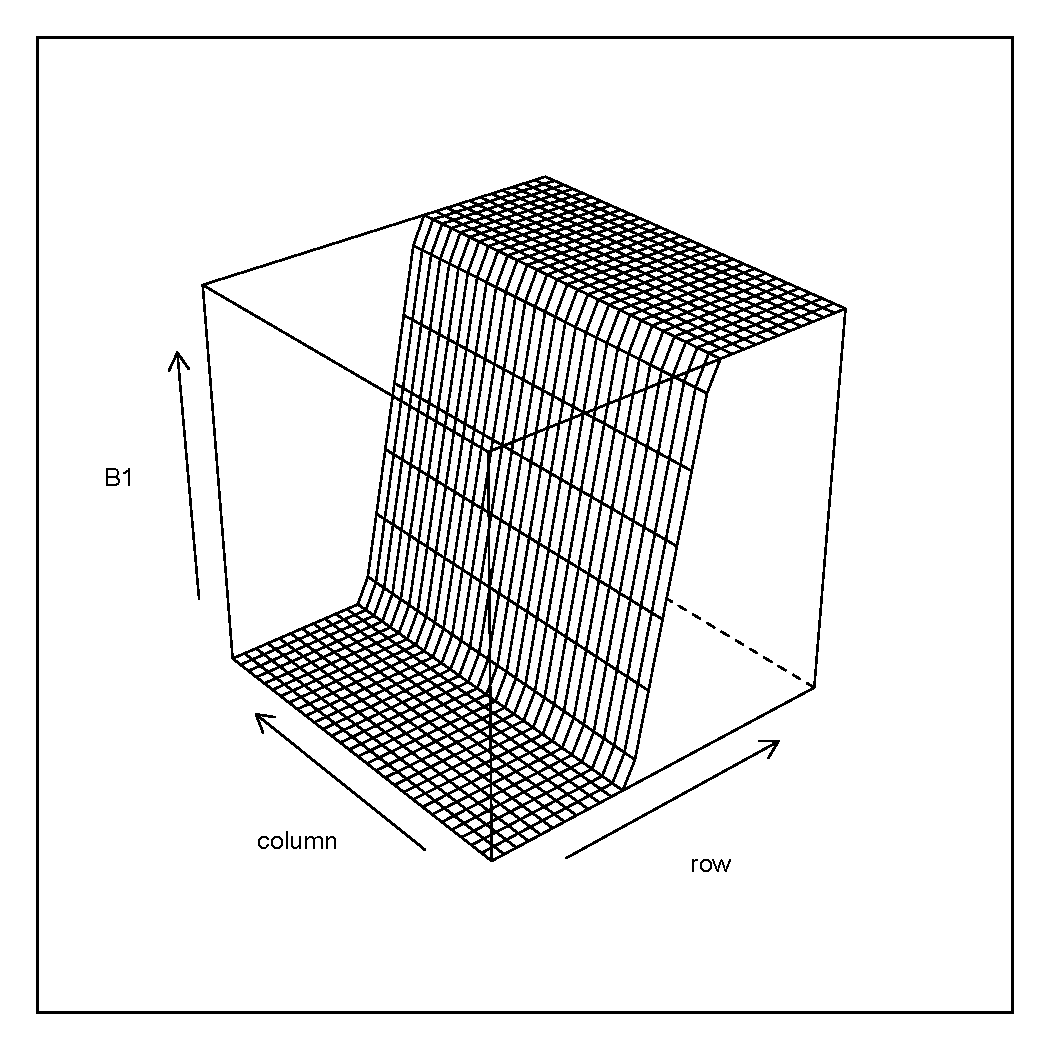
\includegraphics[width=0.32\textwidth]{../../figures/simulation/step.pdf}
			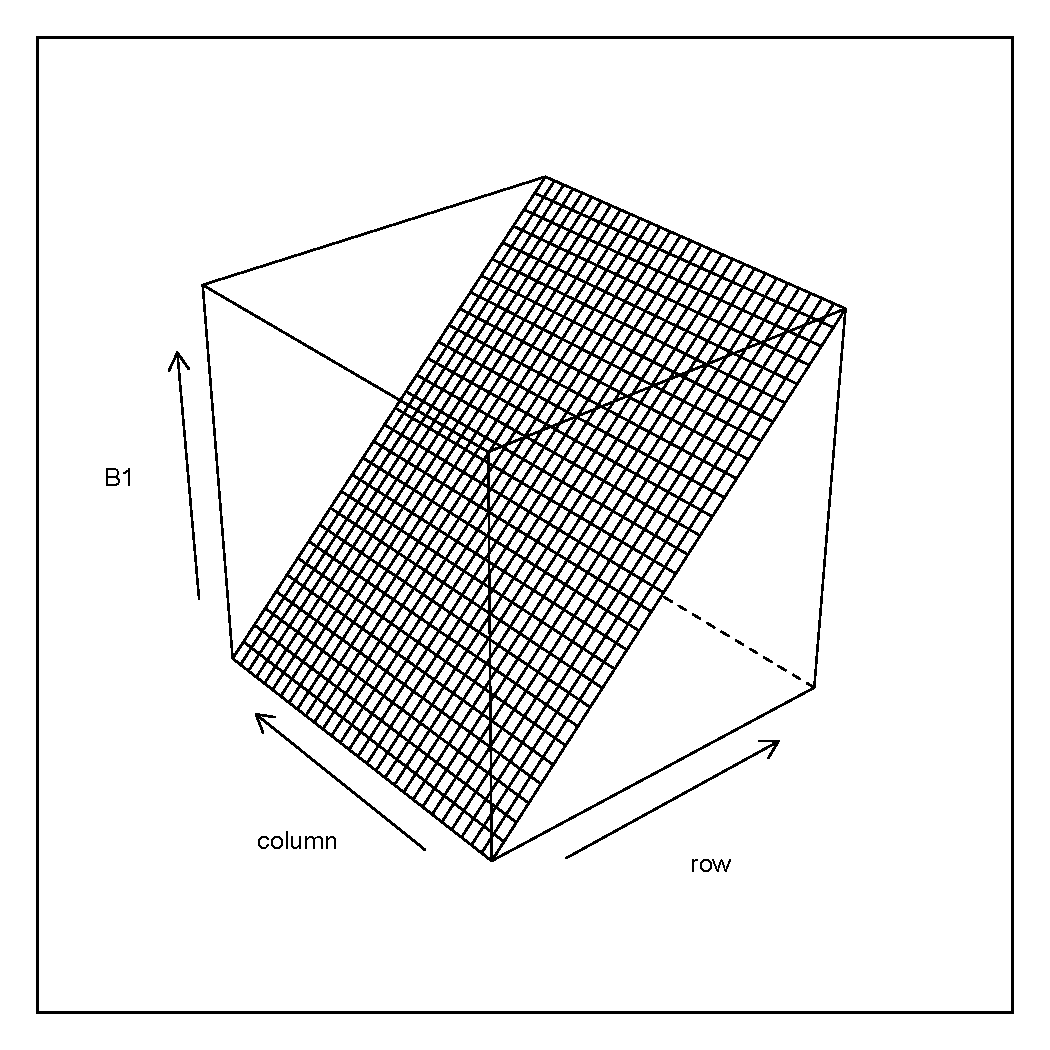
\includegraphics[width=0.32\textwidth]{../../figures/simulation/gradient.pdf}
			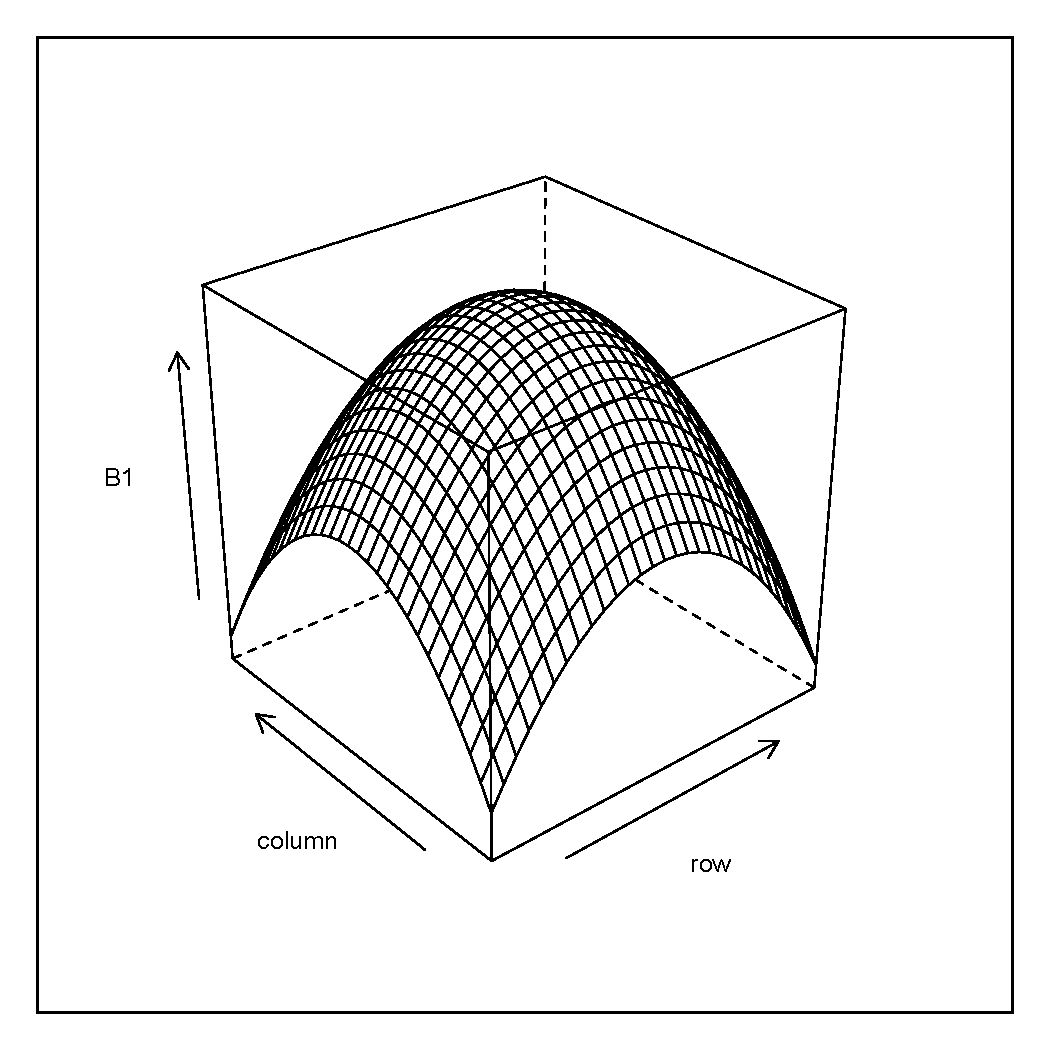
\includegraphics[width=0.32\textwidth]{../../figures/simulation/parabola.pdf}
			\caption{The actual $\beta_1$ coefficient surface used in the simulation.\label{fig:sim-actual}}
		\end{center}
	\end{figure}
	
	\subsection{Results}
	Results from the simulation were summarized at five locations on the simulated grid. The five key locations were chosen because they represent interesting regions of the $\beta_1$ coefficient surface. The results of variable selection (Tables \ref{table:loc1-selection} - \ref{table:loc5-selection}) and coefficient estimation (Tables \ref{table:loc1-X1-MSEX} - \ref{table:loc5-estimation}) are presented in the tables below.
	%Results of the simulation experiment were summarized to asses the consistency in selection and estimation, as well as the coverage properties of the confidence intervals. The confidence intervals based on the bootstrap (without shrinkage) were used for the GWL because they seemed to uniformly outperform the other options.\\
	
		
	\subsection{Discussion}
	
	
	
	\subsection{Tables}
		\subsubsection{Selection}
		% latex table generated in R 2.15.2 by xtable 1.7-0 package
		% Thu Apr 18 16:14:00 2013
		\begin{table}[ht]
		\begin{center}
		\begin{tabular}{cc|cc|cc}
		\multicolumn{2}{c}{\texttt{lars}} & \multicolumn{2}{c}{\texttt{enet}} & \multicolumn{2}{c}{\texttt{glmnet}} \\
		 $\beta_1$ & $\beta_4$ - $\beta_5$ & $\beta_1$ & $\beta_4$ - $\beta_5$ & $\beta_1$ & $\beta_4$ - $\beta_5$ \\ 
		  \hline
		0.98 & 0.04 & 1.00 & 0.04 & 1.00 & 0.05 \\ 
		  0.89 & 0.09 & 0.86 & 0.09 & 0.82 & 0.07 \\ 
		  0.96 & 0.07 & 0.99 & 0.10 & 0.96 & 0.09 \\ 
		  0.84 & 0.04 & 0.84 & 0.07 & 0.88 & 0.05 \\ 
		  \hline
		  1.00 & 0.04 & 1.00 & 0.03 & 1.00 & 0.03 \\ 
		  0.99 & 0.08 & 0.97 & 0.07 & 0.97 & 0.07 \\ 
		  1.00 & 0.07 & 1.00 & 0.06 & 1.00 & 0.04 \\ 
		  0.90 & 0.08 & 0.92 & 0.08 & 0.92 & 0.08 \\ 
		  \hline
		  0.94 & 0.06 & 0.95 & 0.06 & 0.94 & 0.06 \\ 
		  0.80 & 0.06 & 0.81 & 0.07 & 0.80 & 0.06 \\ 
		  0.95 & 0.06 & 0.94 & 0.09 & 0.95 & 0.04 \\ 
		  0.78 & 0.12 & 0.79 & 0.12 & 0.80 & 0.12 \\ 
		  \end{tabular}
		\caption{Selection frequency at location 1\label{table:loc1-selection}}
		\end{center}
		\end{table}
		% latex table generated in R 2.15.2 by xtable 1.7-0 package
		% Thu Apr 18 16:14:00 2013
		\begin{table}[ht]
		\begin{center}
		\begin{tabular}{cc|cc|cc}
		\multicolumn{2}{c}{\texttt{lars}} & \multicolumn{2}{c}{\texttt{enet}} & \multicolumn{2}{c}{\texttt{glmnet}} \\
		 $\beta_1$ & $\beta_4$ - $\beta_5$ & $\beta_1$ & $\beta_4$ - $\beta_5$ & $\beta_1$ & $\beta_4$ - $\beta_5$ \\ 
		  \hline
		1.00 & 0.07 & 1.00 & 0.07 & 1.00 & 0.07 \\ 
		  1.00 & 0.06 & 1.00 & 0.06 & 1.00 & 0.07 \\ 
		  1.00 & 0.05 & 1.00 & 0.06 & 1.00 & 0.05 \\ 
		  0.99 & 0.03 & 1.00 & 0.07 & 0.99 & 0.04 \\ 
		  \hline
		  1.00 & 0.10 & 1.00 & 0.08 & 1.00 & 0.07 \\ 
		  0.98 & 0.07 & 0.98 & 0.08 & 0.99 & 0.07 \\ 
		  1.00 & 0.07 & 1.00 & 0.06 & 1.00 & 0.05 \\ 
		  0.98 & 0.06 & 0.99 & 0.08 & 0.99 & 0.05 \\ 
		  \hline
		  1.00 & 0.09 & 1.00 & 0.08 & 1.00 & 0.08 \\ 
		  0.97 & 0.12 & 0.98 & 0.11 & 0.98 & 0.10 \\ 
		  1.00 & 0.06 & 1.00 & 0.05 & 1.00 & 0.05 \\ 
		  0.94 & 0.08 & 0.94 & 0.10 & 0.94 & 0.08 \\ 
		  \end{tabular}
		\caption{Selection frequency at location 2\label{table:loc2-selection}}
		\end{center}
		\end{table}
		% latex table generated in R 2.15.2 by xtable 1.7-0 package
		% Thu Apr 18 16:14:00 2013
		\begin{table}[ht]
		\begin{center}
		\begin{tabular}{cc|cc|cc}
		\multicolumn{2}{c}{\texttt{lars}} & \multicolumn{2}{c}{\texttt{enet}} & \multicolumn{2}{c}{\texttt{glmnet}} \\
		 $\beta_1$ & $\beta_4$ - $\beta_5$ & $\beta_1$ & $\beta_4$ - $\beta_5$ & $\beta_1$ & $\beta_4$ - $\beta_5$ \\ 
		  \hline
		0.99 & 0.05 & 0.99 & 0.06 & 0.99 & 0.06 \\ 
		  0.84 & 0.08 & 0.84 & 0.08 & 0.82 & 0.07 \\ 
		  0.96 & 0.05 & 0.97 & 0.08 & 0.92 & 0.04 \\ 
		  0.78 & 0.08 & 0.81 & 0.11 & 0.80 & 0.08 \\ 
		  \hline
		  1.00 & 0.09 & 1.00 & 0.08 & 1.00 & 0.07 \\ 
		  0.98 & 0.08 & 0.95 & 0.08 & 0.96 & 0.07 \\ 
		  1.00 & 0.07 & 1.00 & 0.06 & 1.00 & 0.04 \\ 
		  0.93 & 0.09 & 0.95 & 0.09 & 0.94 & 0.09 \\ 
		  \hline
		  1.00 & 0.09 & 1.00 & 0.09 & 1.00 & 0.09 \\ 
		  0.96 & 0.10 & 0.97 & 0.09 & 0.97 & 0.10 \\ 
		  1.00 & 0.08 & 1.00 & 0.07 & 1.00 & 0.07 \\ 
		  0.93 & 0.10 & 0.94 & 0.10 & 0.96 & 0.10 \\ 
		  \end{tabular}
		\caption{Selection frequency at location 3\label{table:loc3-selection}}
		\end{center}
		\end{table}
		% latex table generated in R 2.15.2 by xtable 1.7-0 package
		% Thu Apr 18 16:14:00 2013
		\begin{table}[ht]
		\begin{center}
		\begin{tabular}{cc|cc|cc}
		\multicolumn{2}{c}{\texttt{lars}} & \multicolumn{2}{c}{\texttt{enet}} & \multicolumn{2}{c}{\texttt{glmnet}} \\
		 $\beta_1$ & $\beta_4$ - $\beta_5$ & $\beta_1$ & $\beta_4$ - $\beta_5$ & $\beta_1$ & $\beta_4$ - $\beta_5$ \\ 
		  \hline
		0.57 & 0.08 & 0.64 & 0.06 & 0.59 & 0.06 \\ 
		  0.48 & 0.07 & 0.48 & 0.07 & 0.49 & 0.07 \\ 
		  0.45 & 0.08 & 0.51 & 0.12 & 0.40 & 0.07 \\ 
		  0.53 & 0.08 & 0.52 & 0.07 & 0.51 & 0.07 \\ 
		  \hline
		  1.00 & 0.06 & 1.00 & 0.06 & 1.00 & 0.06 \\ 
		  0.98 & 0.07 & 0.95 & 0.07 & 0.93 & 0.06 \\ 
		  1.00 & 0.09 & 1.00 & 0.08 & 1.00 & 0.10 \\ 
		  0.96 & 0.07 & 0.95 & 0.11 & 0.95 & 0.08 \\ 
		  \hline
		  1.00 & 0.09 & 1.00 & 0.08 & 1.00 & 0.08 \\ 
		  0.93 & 0.07 & 0.92 & 0.08 & 0.94 & 0.08 \\ 
		  1.00 & 0.08 & 1.00 & 0.08 & 1.00 & 0.08 \\ 
		  0.96 & 0.08 & 0.96 & 0.09 & 0.96 & 0.09 \\ 
		  \end{tabular}
		\caption{Selection frequency at location 4\label{table:loc4-selection}}
		\end{center}
		\end{table}
		% latex table generated in R 2.15.2 by xtable 1.7-0 package
		% Thu Apr 18 16:14:00 2013
		\begin{table}[ht]
		\begin{center}
		\begin{tabular}{cc|cc|cc}
		\multicolumn{2}{c}{\texttt{lars}} & \multicolumn{2}{c}{\texttt{enet}} & \multicolumn{2}{c}{\texttt{glmnet}} \\
		 $\beta_1$ & $\beta_4$ - $\beta_5$ & $\beta_1$ & $\beta_4$ - $\beta_5$ & $\beta_1$ & $\beta_4$ - $\beta_5$ \\ 
		  \hline
		0.04 & 0.03 & 0.03 & 0.03 & 0.03 & 0.03 \\ 
		  0.07 & 0.05 & 0.06 & 0.04 & 0.04 & 0.05 \\ 
		  0.02 & 0.04 & 0.02 & 0.03 & 0.03 & 0.05 \\ 
		  0.05 & 0.04 & 0.04 & 0.03 & 0.06 & 0.06 \\ 
		  \hline
		  0.92 & 0.05 & 0.93 & 0.05 & 0.94 & 0.04 \\ 
		  0.71 & 0.08 & 0.70 & 0.07 & 0.70 & 0.07 \\ 
		  0.93 & 0.10 & 0.95 & 0.14 & 0.95 & 0.10 \\ 
		  0.60 & 0.07 & 0.63 & 0.13 & 0.64 & 0.06 \\ 
		  \hline
		  0.93 & 0.10 & 0.93 & 0.09 & 0.92 & 0.10 \\ 
		  0.80 & 0.05 & 0.81 & 0.05 & 0.79 & 0.05 \\ 
		  0.93 & 0.07 & 0.94 & 0.12 & 0.94 & 0.07 \\ 
		  0.81 & 0.09 & 0.81 & 0.11 & 0.83 & 0.08 \\ 
		  \end{tabular}
		\caption{Selection frequency at location 5\label{table:loc5-selection}}
		\end{center}
		\end{table}
		

		\subsubsection{Estimation}
		% latex table generated in R 2.15.2 by xtable 1.7-0 package
		% Thu Apr 18 14:39:33 2013
		\begin{table}[ht]
		\begin{center}
		\begin{tabular}{cccccccc}
		 lars & enet & glmnet & unshrunk.lars & unshrunk.enet & unshrunk.glmnet & oracular & gwr \\ 
		  \hline
		0.046 & 0.025 & \emph{0.023} & 0.151 & 0.127 & 0.124 & 0.082 & \textbf{0.005} \\ 
		  0.146 & 0.186 & 0.216 & 0.290 & 0.376 & 0.375 & \emph{0.134} & \textbf{0.009} \\ 
		  0.072 & \emph{0.045} & 0.073 & 0.172 & 0.134 & 0.205 & 0.101 & \textbf{0.011} \\ 
		  0.214 & 0.218 & 0.179 & 0.441 & 0.425 & 0.369 & \emph{0.154} & \textbf{0.022} \\ 
		  0.066 & 0.069 & 0.070 & 0.007 & \textbf{0.007} & \emph{0.007} & 0.010 & 0.016 \\ 
		  0.084 & 0.094 & 0.096 & 0.161 & 0.078 & 0.085 & \emph{0.045} & \textbf{0.042} \\ 
		  0.065 & 0.070 & 0.069 & 0.009 & \textbf{0.007} & \emph{0.008} & 0.009 & 0.019 \\ 
		  0.161 & 0.149 & 0.144 & 0.149 & 0.123 & 0.121 & \textbf{0.040} & \emph{0.050} \\ 
		  0.074 & 0.075 & 0.074 & 0.020 & \emph{0.020} & \textbf{0.020} & 0.022 & 0.105 \\ 
		  0.079 & 0.078 & 0.077 & 0.041 & \emph{0.040} & \textbf{0.039} & 0.063 & 0.106 \\ 
		  0.077 & 0.069 & 0.076 & 0.024 & \textbf{0.018} & 0.023 & \emph{0.023} & 0.099 \\ 
		  0.083 & 0.072 & 0.083 & \emph{0.048} & \textbf{0.044} & 0.050 & 0.067 & 0.110 \\ 
		  \end{tabular}
		\caption{Mean squared error of estimates for $\beta_1$ at location 1 (\textbf{minimum}, \emph{next best}).\label{loc1-X1-MSEX}}
		\end{center}
		\end{table}
		
		% latex table generated in R 2.15.2 by xtable 1.7-0 package
		% Thu Apr 18 14:39:33 2013
		\begin{table}[ht]
		\begin{center}
		\begin{tabular}{cccccccc}
		 lars & enet & glmnet & unshrunk.lars & unshrunk.enet & unshrunk.glmnet & oracular & gwr \\ 
		  \hline
		0.024 & 0.024 & 0.024 & \textbf{0.020} & 0.021 & \emph{0.021} & 0.021 & 0.042 \\ 
		  0.061 & 0.063 & 0.068 & \emph{0.050} & 0.054 & 0.056 & \textbf{0.042} & 0.070 \\ 
		  0.022 & 0.027 & 0.021 & \textbf{0.017} & 0.021 & \emph{0.017} & 0.018 & 0.044 \\ 
		  0.069 & 0.071 & 0.071 & 0.057 & \emph{0.056} & 0.061 & \textbf{0.043} & 0.075 \\ 
		  0.003 & 0.003 & 0.003 & \emph{0.001} & 0.001 & 0.001 & \textbf{0.001} & 0.001 \\ 
		  0.014 & 0.013 & 0.008 & 0.015 & 0.013 & 0.009 & \emph{0.002} & \textbf{0.002} \\ 
		  0.003 & 0.003 & 0.003 & 0.001 & \emph{0.001} & \textbf{0.001} & 0.001 & 0.002 \\ 
		  0.015 & 0.012 & 0.012 & 0.014 & 0.011 & 0.011 & \textbf{0.003} & \emph{0.004} \\ 
		  \emph{0.005} & 0.005 & 0.005 & 0.007 & 0.007 & 0.007 & \textbf{0.004} & 0.007 \\ 
		  0.018 & 0.016 & 0.016 & 0.026 & 0.021 & 0.022 & \emph{0.008} & \textbf{0.007} \\ 
		  0.007 & 0.007 & \emph{0.007} & 0.011 & 0.010 & 0.009 & \textbf{0.004} & 0.008 \\ 
		  0.020 & 0.022 & 0.020 & 0.022 & 0.022 & 0.023 & \textbf{0.007} & \emph{0.009} \\ 
		  \end{tabular}
		\caption{Mean squared error of estimates for $\beta_1$ at location 2 (\textbf{minimum}, \emph{next best}).\label{loc2-X1-MSEX}}
		\end{center}
		\end{table}
		
		% latex table generated in R 2.15.2 by xtable 1.7-0 package
		% Thu Apr 18 14:39:33 2013
		\begin{table}[ht]
		\begin{center}
		\begin{tabular}{cccccccc}
		 lars & enet & glmnet & unshrunk.lars & unshrunk.enet & unshrunk.glmnet & oracular & gwr \\ 
		  \hline
		0.011 & 0.011 & 0.010 & 0.007 & 0.007 & 0.007 & \textbf{0.004} & \emph{0.005} \\ 
		  0.043 & 0.043 & 0.047 & 0.049 & 0.049 & 0.054 & \emph{0.009} & \textbf{0.008} \\ 
		  0.016 & 0.014 & 0.022 & 0.013 & 0.011 & 0.021 & \textbf{0.005} & \emph{0.005} \\ 
		  0.048 & 0.047 & 0.045 & 0.049 & 0.045 & 0.044 & \emph{0.008} & \textbf{0.008} \\ 
		  0.001 & 0.001 & 0.001 & \textbf{0.001} & 0.001 & 0.001 & \emph{0.001} & 0.001 \\ 
		  0.007 & 0.017 & 0.015 & 0.007 & 0.019 & 0.017 & \emph{0.002} & \textbf{0.002} \\ 
		  0.001 & 0.001 & 0.000 & 0.000 & \emph{0.000} & \textbf{0.000} & 0.001 & 0.002 \\ 
		  0.022 & 0.017 & 0.019 & 0.023 & 0.017 & 0.021 & \textbf{0.002} & \emph{0.003} \\ 
		  0.015 & 0.015 & 0.015 & 0.015 & 0.015 & \emph{0.015} & \textbf{0.005} & 0.022 \\ 
		  0.032 & 0.029 & 0.029 & 0.030 & 0.027 & 0.027 & \textbf{0.012} & \emph{0.023} \\ 
		  0.019 & 0.018 & 0.019 & 0.018 & \emph{0.017} & 0.018 & \textbf{0.005} & 0.024 \\ 
		  0.037 & 0.037 & 0.030 & 0.037 & 0.034 & 0.029 & \textbf{0.012} & \emph{0.024} \\ 
		  \end{tabular}
		\caption{Mean squared error of estimates for $\beta_1$ at location 3 (\textbf{minimum}, \emph{next best}).\label{loc3-X1-MSEX}}
		\end{center}
		\end{table}
		
		% latex table generated in R 2.15.2 by xtable 1.7-0 package
		% Thu Apr 18 14:39:33 2013
		\begin{table}[ht]
		\begin{center}
		\begin{tabular}{cccccccc}
		 lars & enet & glmnet & unshrunk.lars & unshrunk.enet & unshrunk.glmnet & oracular & gwr \\ 
		  \hline
		\emph{0.014} & 0.014 & \textbf{0.014} & 0.017 & 0.019 & 0.018 & 0.021 & 0.042 \\ 
		  \emph{0.037} & \textbf{0.036} & 0.039 & 0.039 & 0.042 & 0.046 & 0.047 & 0.074 \\ 
		  \textbf{0.010} & 0.012 & \emph{0.011} & 0.013 & 0.016 & 0.014 & 0.020 & 0.044 \\ 
		  \emph{0.038} & \textbf{0.028} & 0.038 & 0.048 & 0.047 & 0.048 & 0.043 & 0.082 \\ 
		  0.003 & 0.003 & 0.003 & 0.002 & 0.001 & \emph{0.001} & \textbf{0.001} & 0.001 \\ 
		  0.009 & 0.014 & 0.016 & 0.007 & 0.012 & 0.015 & \textbf{0.002} & \emph{0.003} \\ 
		  0.003 & 0.002 & 0.003 & 0.002 & 0.001 & \emph{0.001} & \textbf{0.001} & 0.002 \\ 
		  0.013 & 0.015 & 0.014 & 0.013 & 0.014 & 0.014 & \textbf{0.003} & \emph{0.004} \\ 
		  0.006 & 0.006 & \emph{0.006} & 0.009 & 0.009 & 0.009 & \textbf{0.004} & 0.008 \\ 
		  0.025 & 0.027 & 0.023 & 0.027 & 0.029 & 0.024 & \emph{0.010} & \textbf{0.009} \\ 
		  \emph{0.008} & 0.008 & 0.008 & 0.011 & 0.011 & 0.011 & \textbf{0.004} & 0.010 \\ 
		  0.018 & 0.020 & 0.017 & 0.022 & 0.022 & 0.022 & \textbf{0.009} & \emph{0.010} \\ 
		  \end{tabular}
		\caption{Mean squared error of estimates for $\beta_1$ at location 4 (\textbf{minimum}, \emph{next best}).\label{loc4-X1-MSEX}}
		\end{center}
		\end{table}
		
		% latex table generated in R 2.15.2 by xtable 1.7-0 package
		% Thu Apr 18 14:39:33 2013
		\begin{table}[ht]
		\begin{center}
		\begin{tabular}{cccccccc}
		 lars & enet & glmnet & unshrunk.lars & unshrunk.enet & unshrunk.glmnet & oracular & gwr \\ 
		  \hline
		0.002 & \emph{0.001} & 0.002 & 0.006 & 0.004 & 0.004 & \textbf{0.000} & 0.007 \\ 
		  0.003 & 0.006 & \emph{0.002} & 0.016 & 0.024 & 0.009 & \textbf{0.000} & 0.011 \\ 
		  \emph{0.002} & 0.002 & 0.003 & 0.009 & 0.009 & 0.009 & \textbf{0.000} & 0.010 \\ 
		  0.017 & \emph{0.004} & 0.022 & 0.046 & 0.038 & 0.043 & \textbf{0.000} & 0.015 \\ 
		  0.067 & 0.068 & 0.069 & 0.004 & 0.004 & \emph{0.004} & \textbf{0.000} & 0.016 \\ 
		  0.054 & 0.051 & 0.052 & \emph{0.019} & 0.019 & 0.019 & \textbf{0.000} & 0.044 \\ 
		  0.062 & 0.060 & 0.064 & 0.009 & 0.010 & \emph{0.007} & \textbf{0.000} & 0.021 \\ 
		  0.050 & 0.047 & 0.053 & \emph{0.017} & 0.020 & 0.017 & \textbf{0.000} & 0.051 \\ 
		  0.074 & 0.075 & 0.075 & \textbf{0.018} & 0.020 & 0.021 & \emph{0.020} & 0.104 \\ 
		  0.075 & 0.074 & 0.073 & 0.024 & \textbf{0.022} & \emph{0.023} & 0.055 & 0.104 \\ 
		  0.077 & 0.069 & 0.076 & \emph{0.021} & 0.023 & \textbf{0.020} & 0.025 & 0.099 \\ 
		  0.081 & 0.075 & 0.081 & 0.037 & \emph{0.036} & \textbf{0.035} & 0.042 & 0.113 \\ 
		  \end{tabular}
		\caption{Mean squared error of estimates for $\beta_1$ at location 5 (\textbf{minimum}, \emph{next best}).\label{loc5-X1-MSEX}}
		\end{center}
		\end{table}



	%\subsection{Figures}
	%The plots of bias demonstrate that GWL tended to ``fill the valleys" and ``trim the peaks" of the coefficient surface for $\beta_1$, which is not unexpected for a smoother like GWR. 
	
	%Figures \ref{fig:coveragemap1} - \ref{fig:coveragemap18} show the frequency with which the true value of the parameter $\beta_1$ was covered by the 95\% confidence intervals at each location under each simulation setting. The left column shows the coverage frequency of the 95\% CI of the GWL using the unshrunk-bootstrap method of CI construction. The middle column is the coverage frequency of the 95\% CI the O-GWR using the bootstrap to generate the CI. The right column is the relative efficiency of the GWL to O-GWR. In the first two columns, the color white is used to indicate areas where the nominal coverage frequency of 95\% is achieved, while blue codes areas that exceeded 95\% coverage and orange codes areas that fell short of 95\% coverage. In the third column, the color white indicates areas where the relative efficiency is unity, while orange indicates areas where the relative efficiency was less than unity and blue indicates areas where the relative efficiency exceeded unity.\\	

	


			
\section{Data analysis}
	\subsection{Census poverty data}
	An example analysis is presented to demonstrate application of the geographically-weighted lasso. The analysis focuses on creating a varying-coefficients regression model to describe how poverty is related to a list of demographic and social variables. The data is from the U.S. Census Bureau's decennial census  from 1990. This analysis looks specifically at the upper midwest states of Minnesota, Iowa, Wisconsin, Illinois, Indiana, and Michigan. All data is aggregated at the county level.
	
	Table \ref{table:census-vars} lists the variables that were considered as potential predictors of county-level poverty rate. The outcome of interest (poverty rate) is a proportion and so takes values on $[0,1]$, but to demonstrate the geographically-weighted lasso in a linear regression context, we model the logit-transformed poverty rate. The predictor variables were not transformed - county-level proportions were used.
	
	\begin{table}
		\begin{center}
		\begin{tabular}{ll}
			Variable name & Description \\
			\hline
			\verb!pag! & Proportion working in agriculture\\
			\verb!pex! &  Proportion working in extraction (mining)\\
			\verb!pman! & Proportion working in manufacturing \\
			\verb!pserve! & Proportion working in services \\
			\verb!pfire! & Proportion working in finance, insurance, and real estate \\
			\verb!potprof! & Proportion working in other professions \\
			\verb!pwh! & Proportion who are white \\
			\verb!pblk! & Proportion who are black \\
			\verb!phisp! & Proportion who are hispanic \\
			\verb!metro! & Is the county in a metropolitan area?\\
		\end{tabular}
		\caption{Description of the variables used in the census-data example\label{table:census-vars}}
		\end{center}		
	\end{table}
	
	\subsection{Modeling}	
	Variable selection and coefficient estimation using the geographically-weighted lasso were done for each census separately (no attempt is made here to borrow strength across years). Therefore the bandwidth was chosen independently for the model of each census. Table \ref{table:census-bandwidth} lists the bandwidth that were selected for each census.
	
	\begin{table}
		\begin{center}
		\begin{tabular}{ll}
			Year & Bandwidth \\
			\hline
			1960 & 0.033\\
			1970 &  0.381\\
			1980 & 0.122\\
			1990 & 0.802\\
			2000 & 0.854\\
			2006 & 0.976\\
		\end{tabular}
		\caption{Bandwidth selected for each year's model.\label{table:census-bandwidth}}
		\end{center}		
	\end{table}
	
	\subsection{Figures}
	The coefficient estimates are plotted on maps of the upper midwest in Figures \ref{fig:census-coefs-1960} - \ref{fig:census-coefs-2006}. It is immediately apparent that the estimated coefficient surfaces are non-constant for most variables.\\
		
	\begin{figure}
		\begin{center}
			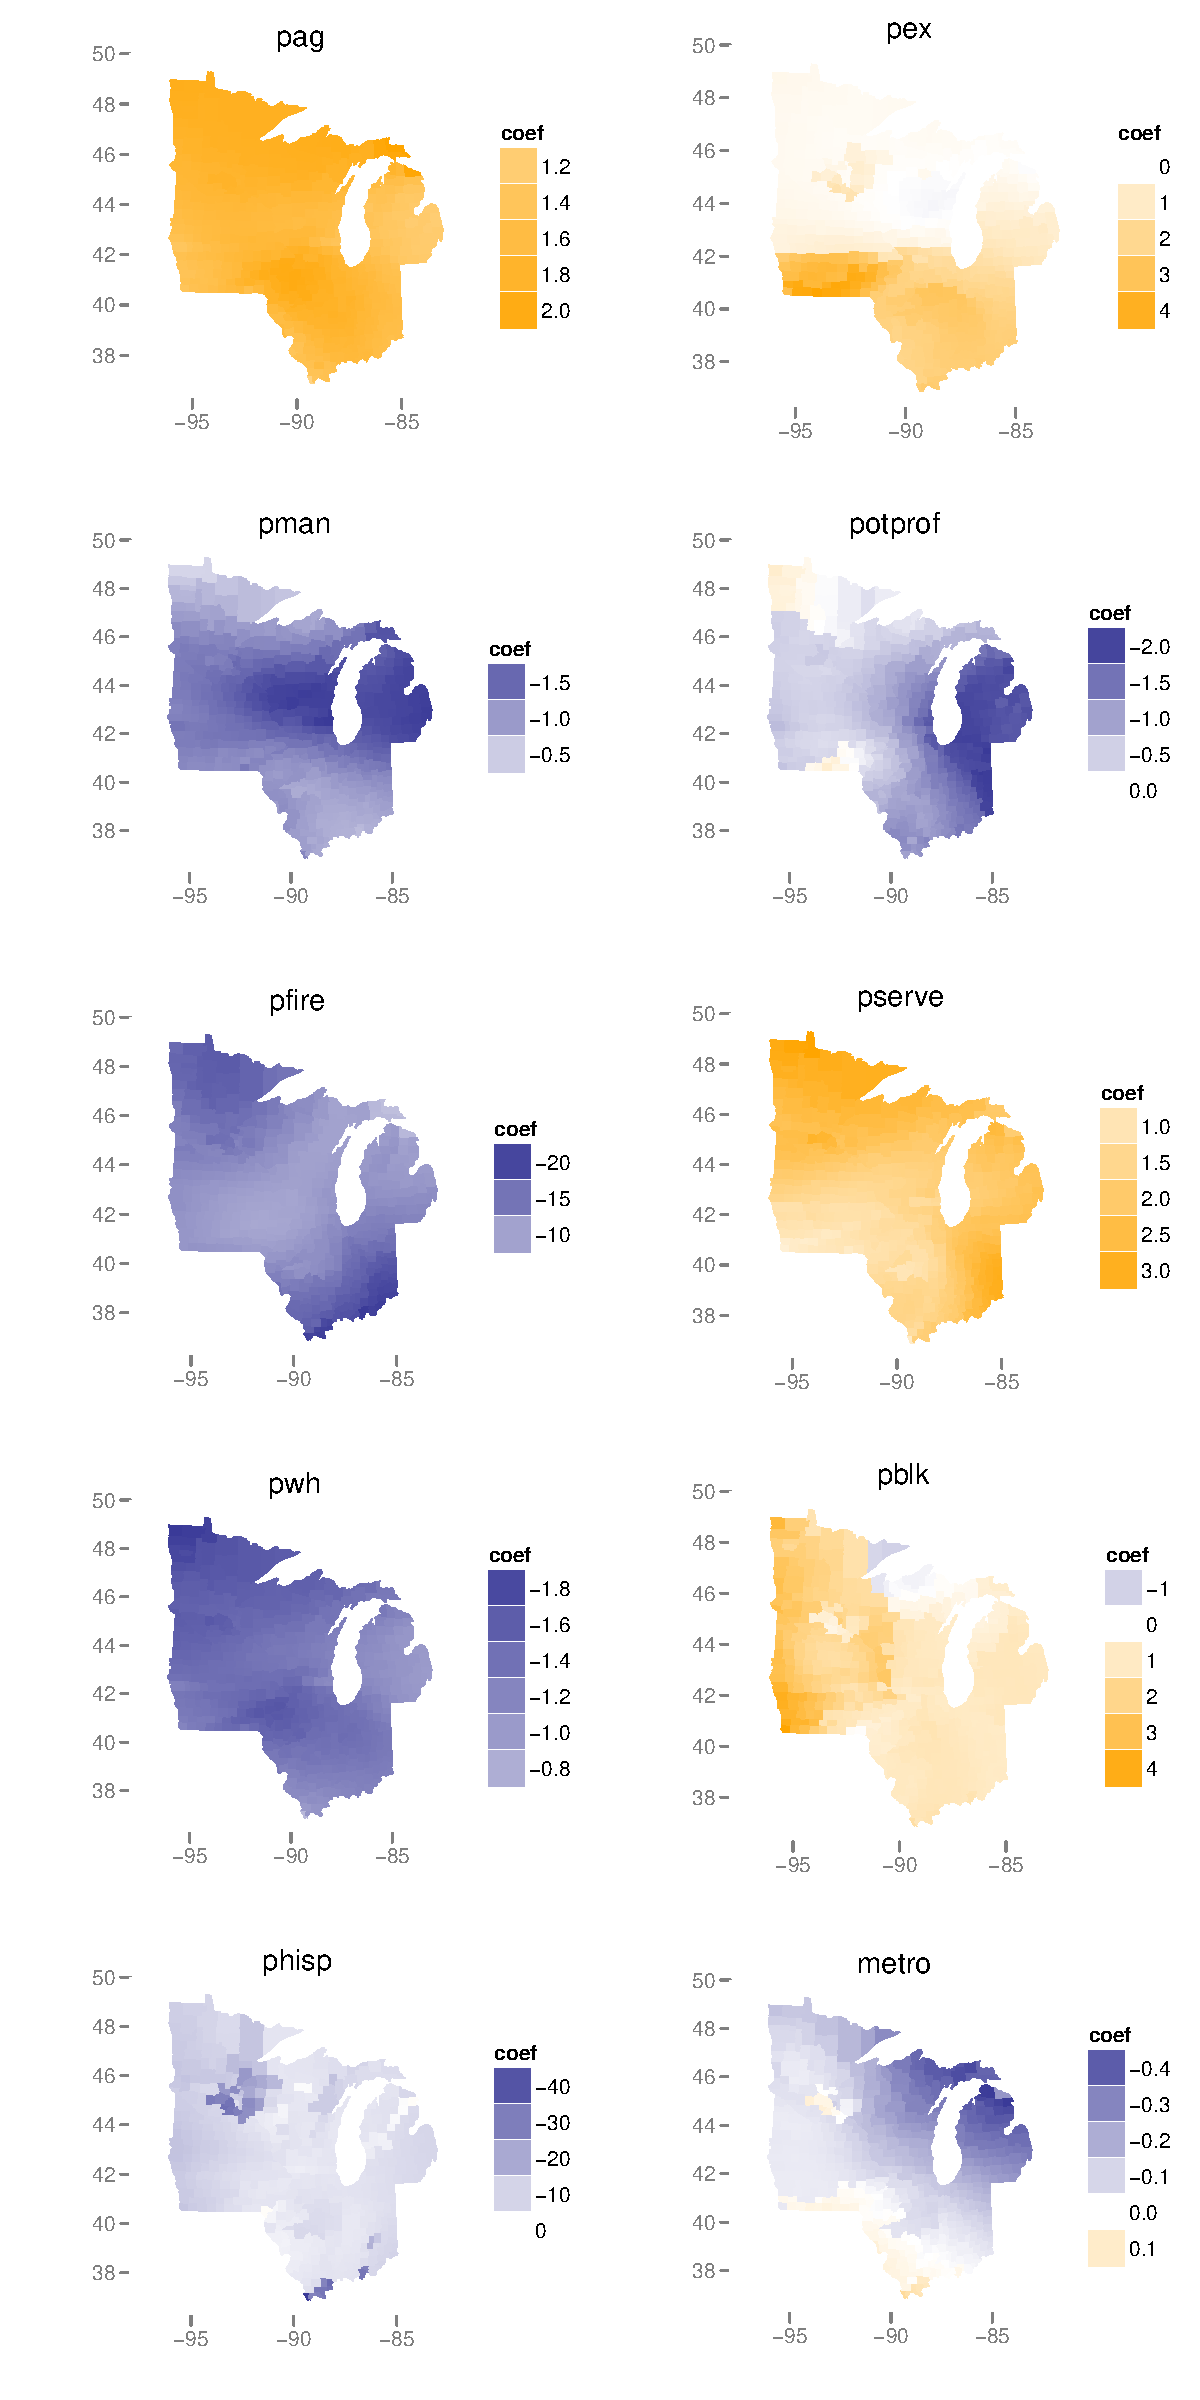
\includegraphics[height=8in]{../../figures/poverty/1960.linear.coefficients.pdf}
			\caption{Estimated coefficient surfaces for the 1960 census.\label{fig:census-coefs-1960}}
		\end{center}		
	\end{figure}

	\begin{figure}
		\begin{center}
			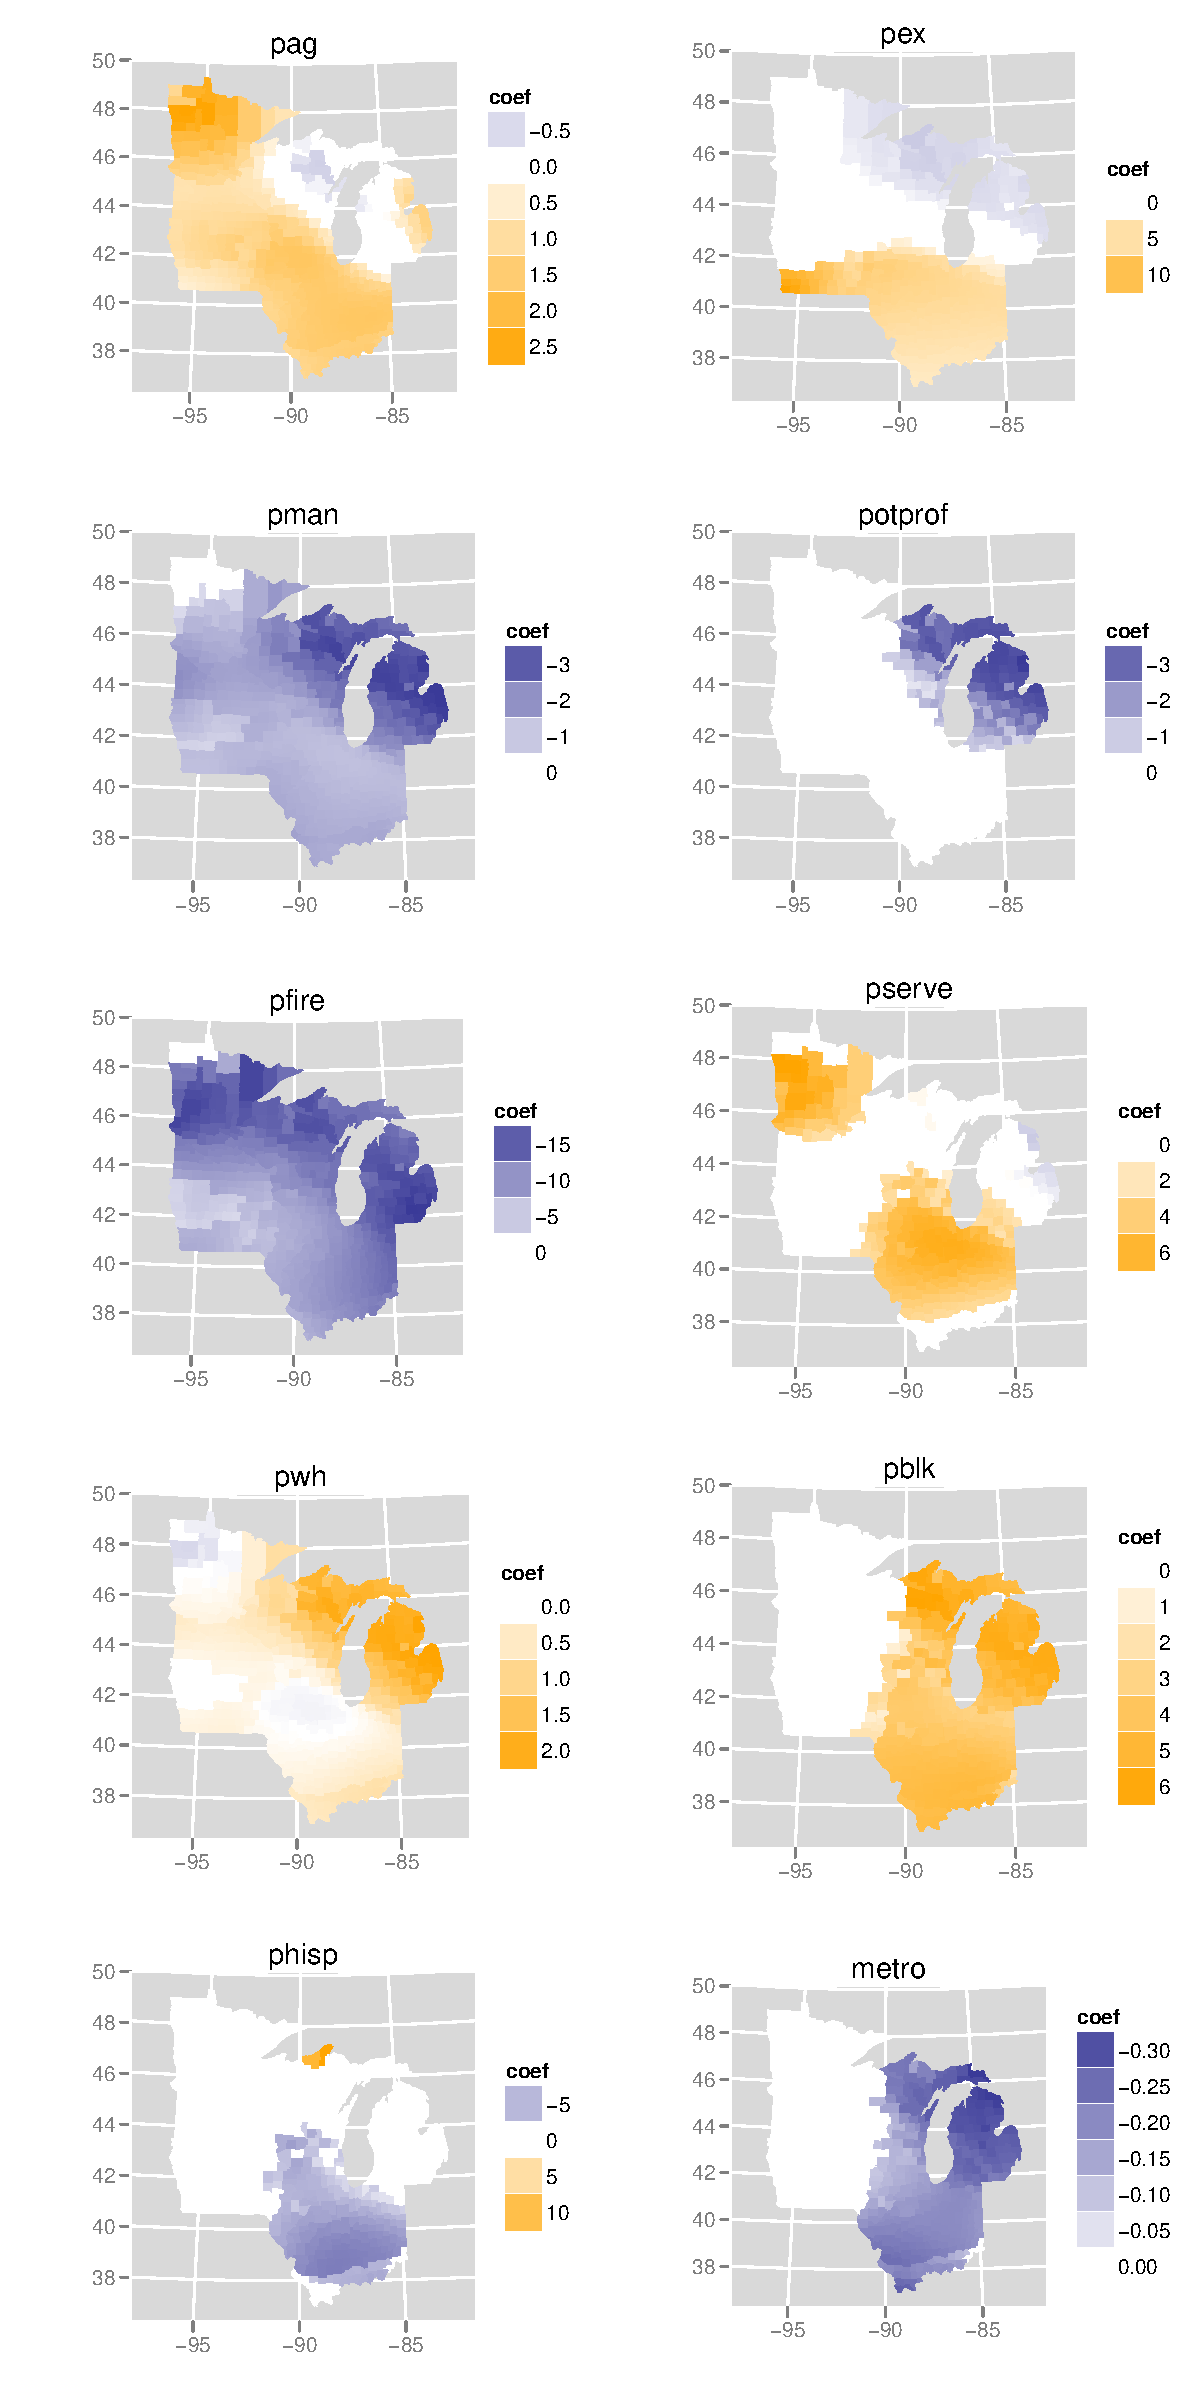
\includegraphics[height=8in]{../../figures/poverty/1970.linear.coefficients.pdf}
			\caption{Estimated coefficient surfaces for the 1970 census.\label{fig:census-coefs-1970}}
		\end{center}
	\end{figure}
	
	\begin{figure}
		\begin{center}
			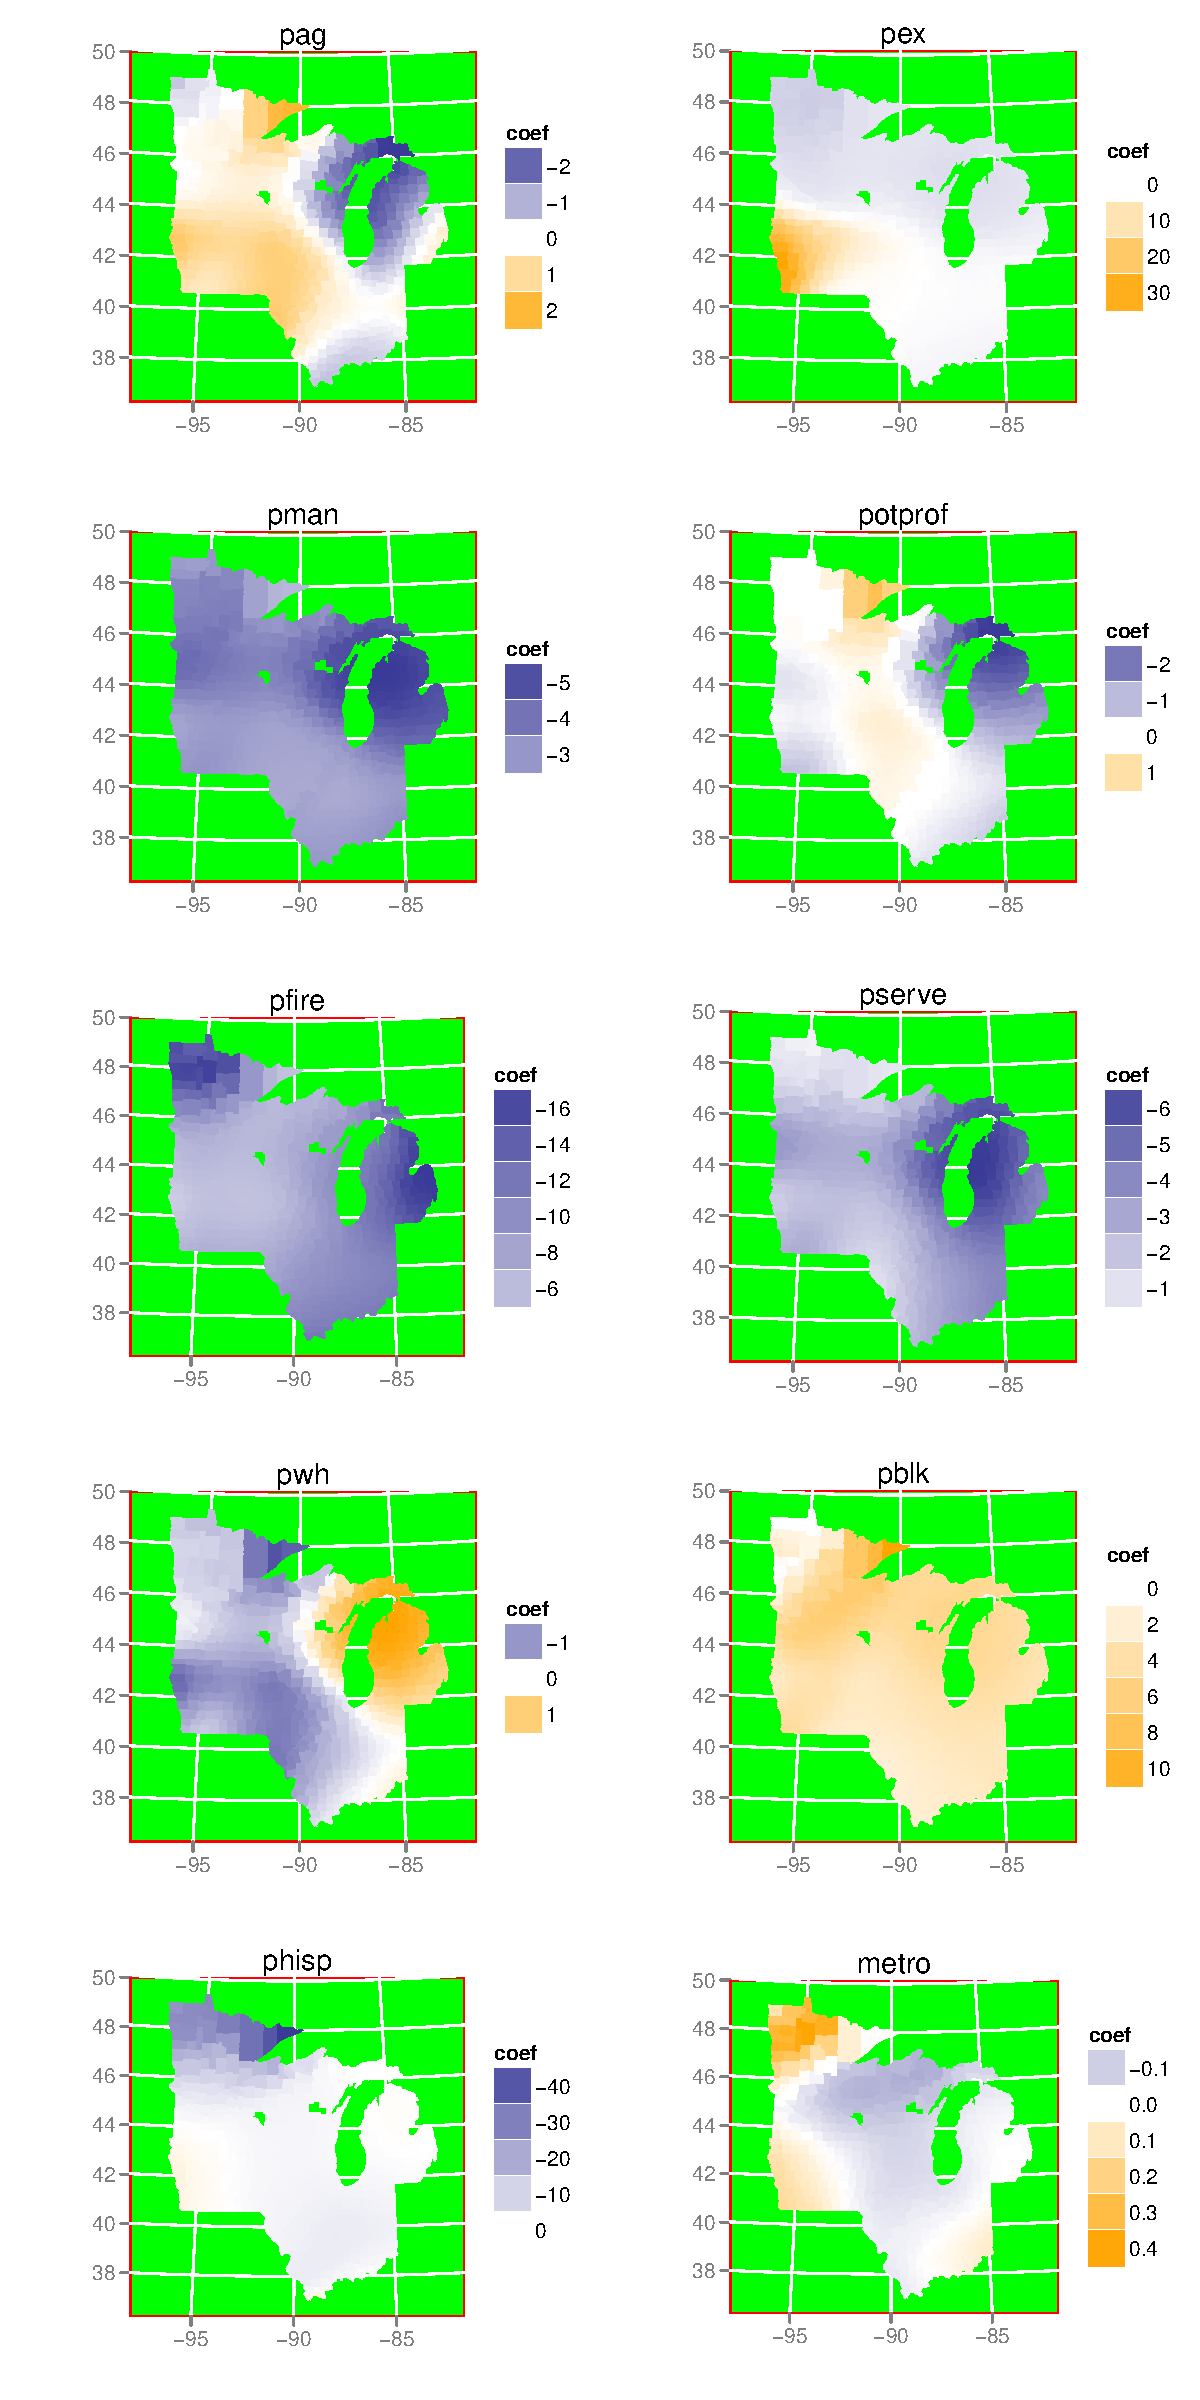
\includegraphics[height=8in]{../../figures/poverty/1980.linear.coefficients.pdf}
			\caption{Estimated coefficient surfaces for the 1980 census.\label{fig:census-coefs-1980}}
		\end{center}
	\end{figure}
	
	\begin{figure}
		\begin{center}
			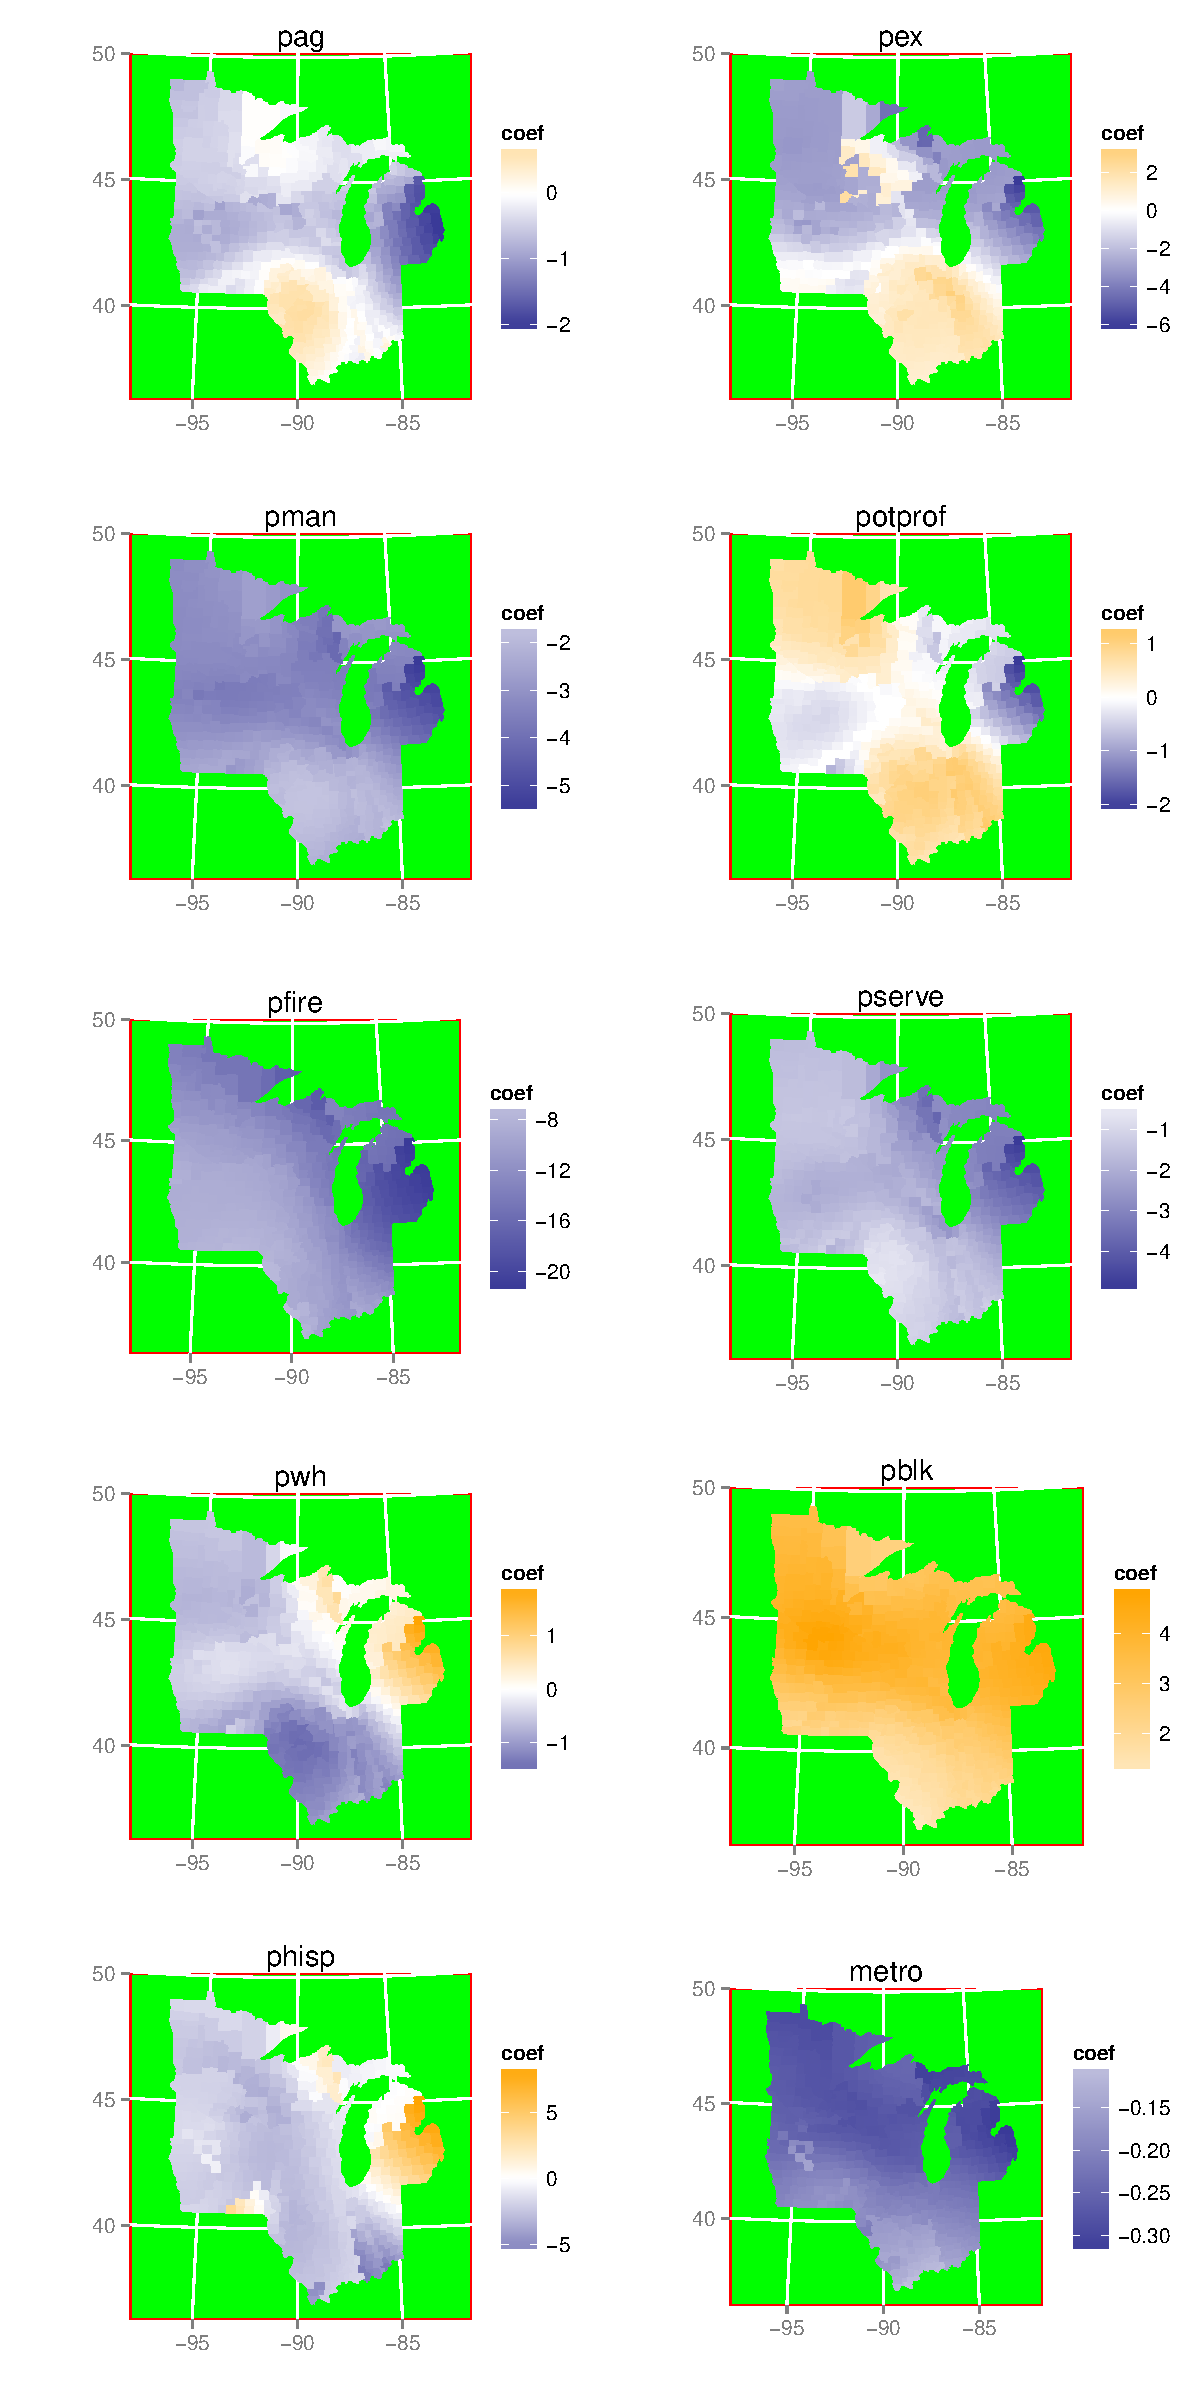
\includegraphics[height=8in]{../../figures/poverty/1990.linear.coefficients.pdf}
			\caption{Estimated coefficient surfaces for the 1990 census.\label{fig:census-coefs-1990}}
		\end{center}
	\end{figure}
	
	\begin{figure}
		\begin{center}
			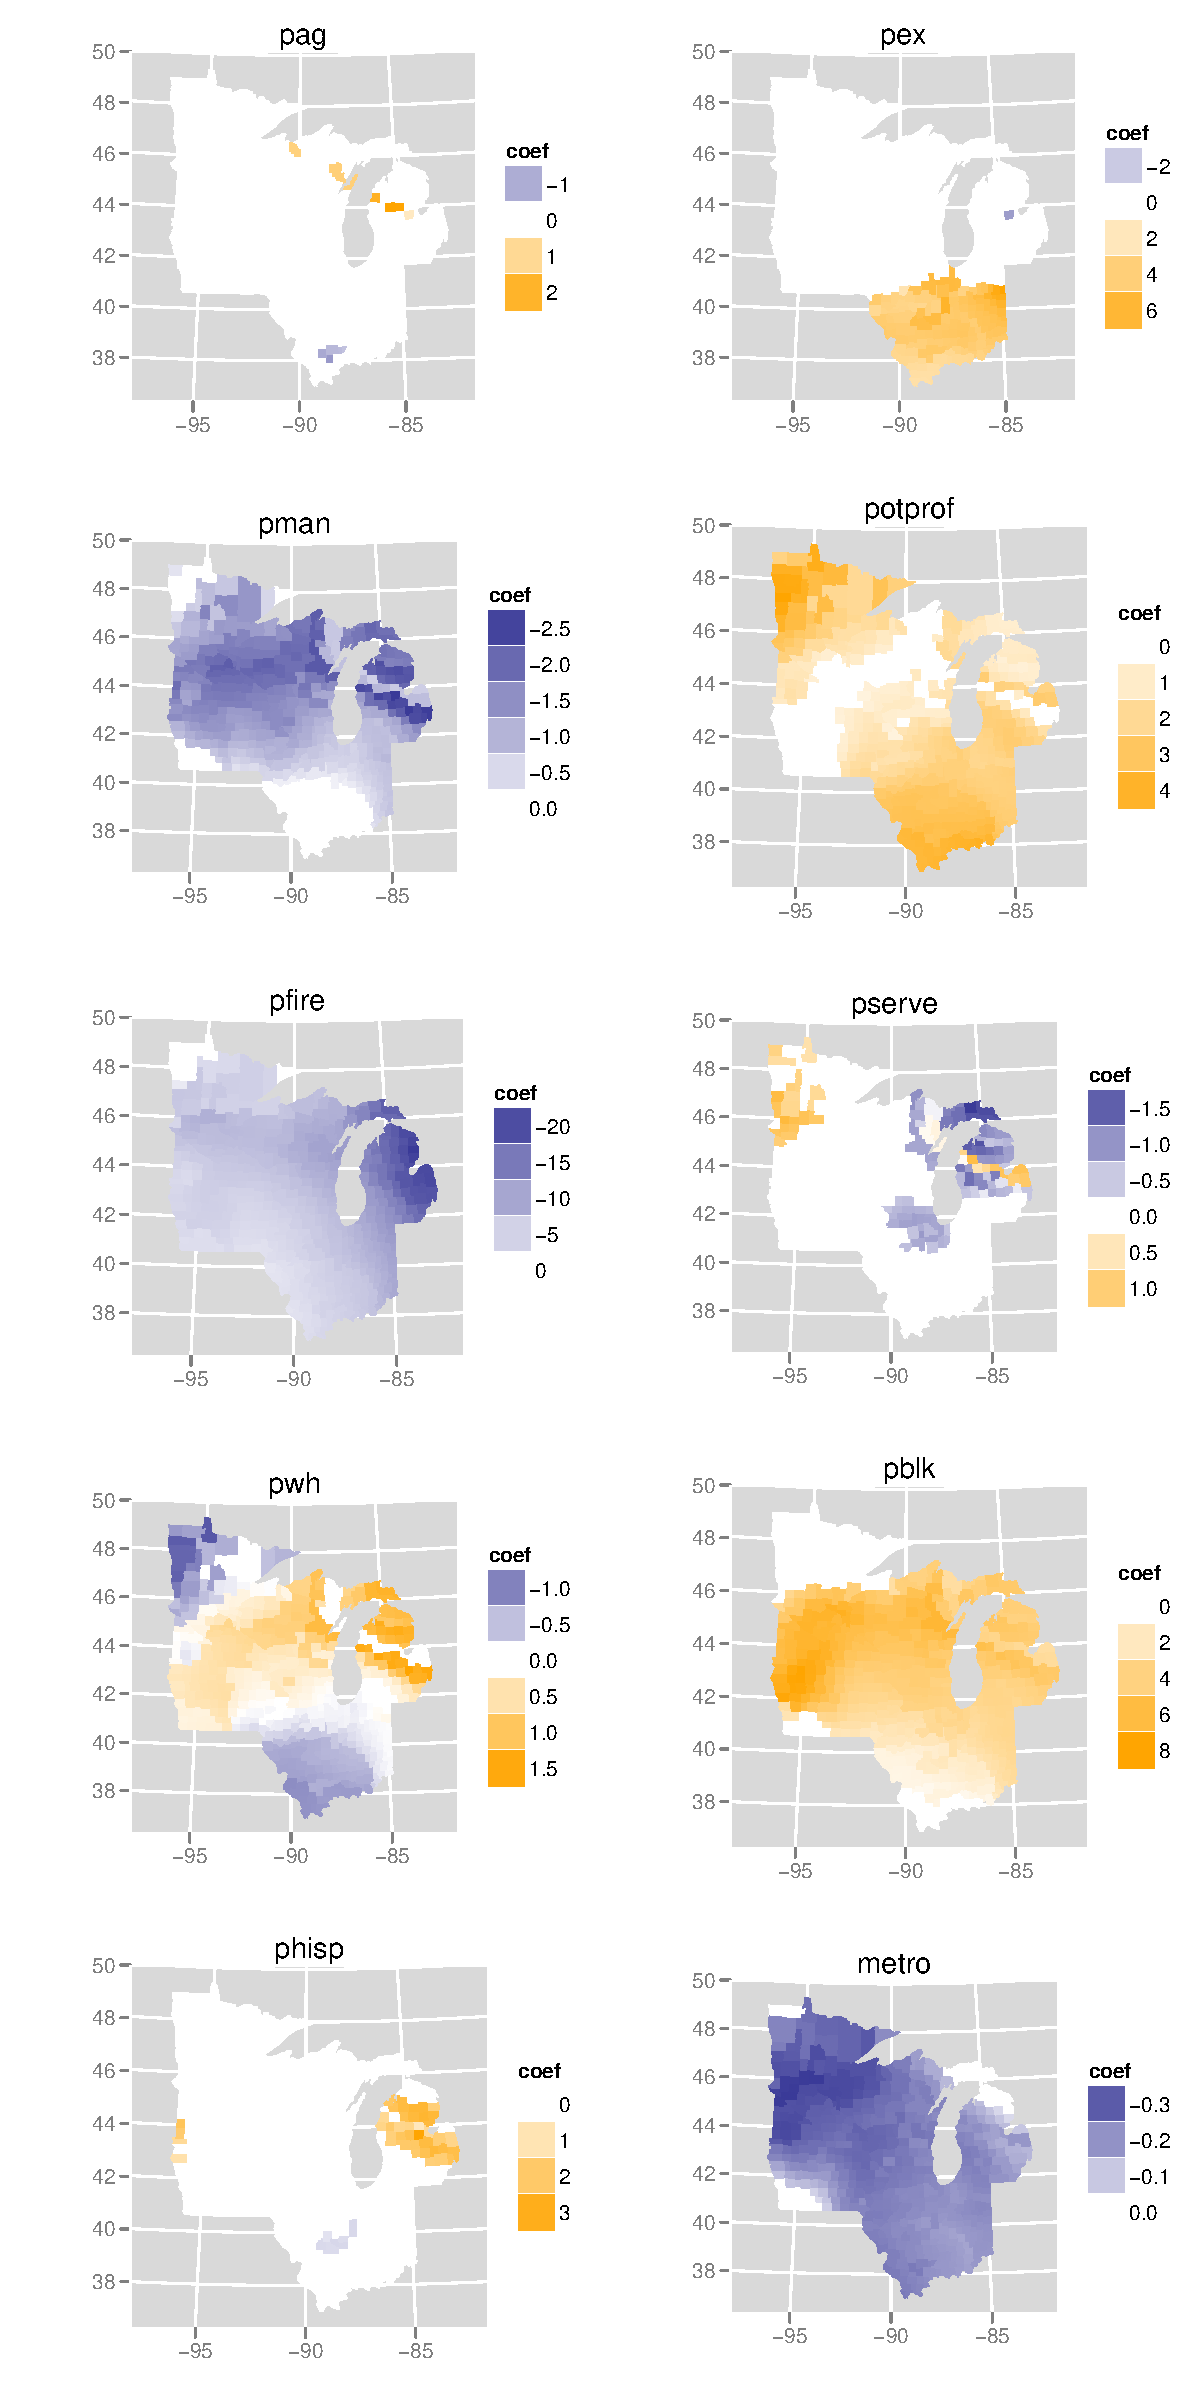
\includegraphics[height=8in]{../../figures/poverty/2000.linear.coefficients.pdf}
			\caption{Estimated coefficient surfaces for the 2000 census.\label{fig:census-coefs-2000}}
		\end{center}
	\end{figure}

	\begin{figure}
		\begin{center}
			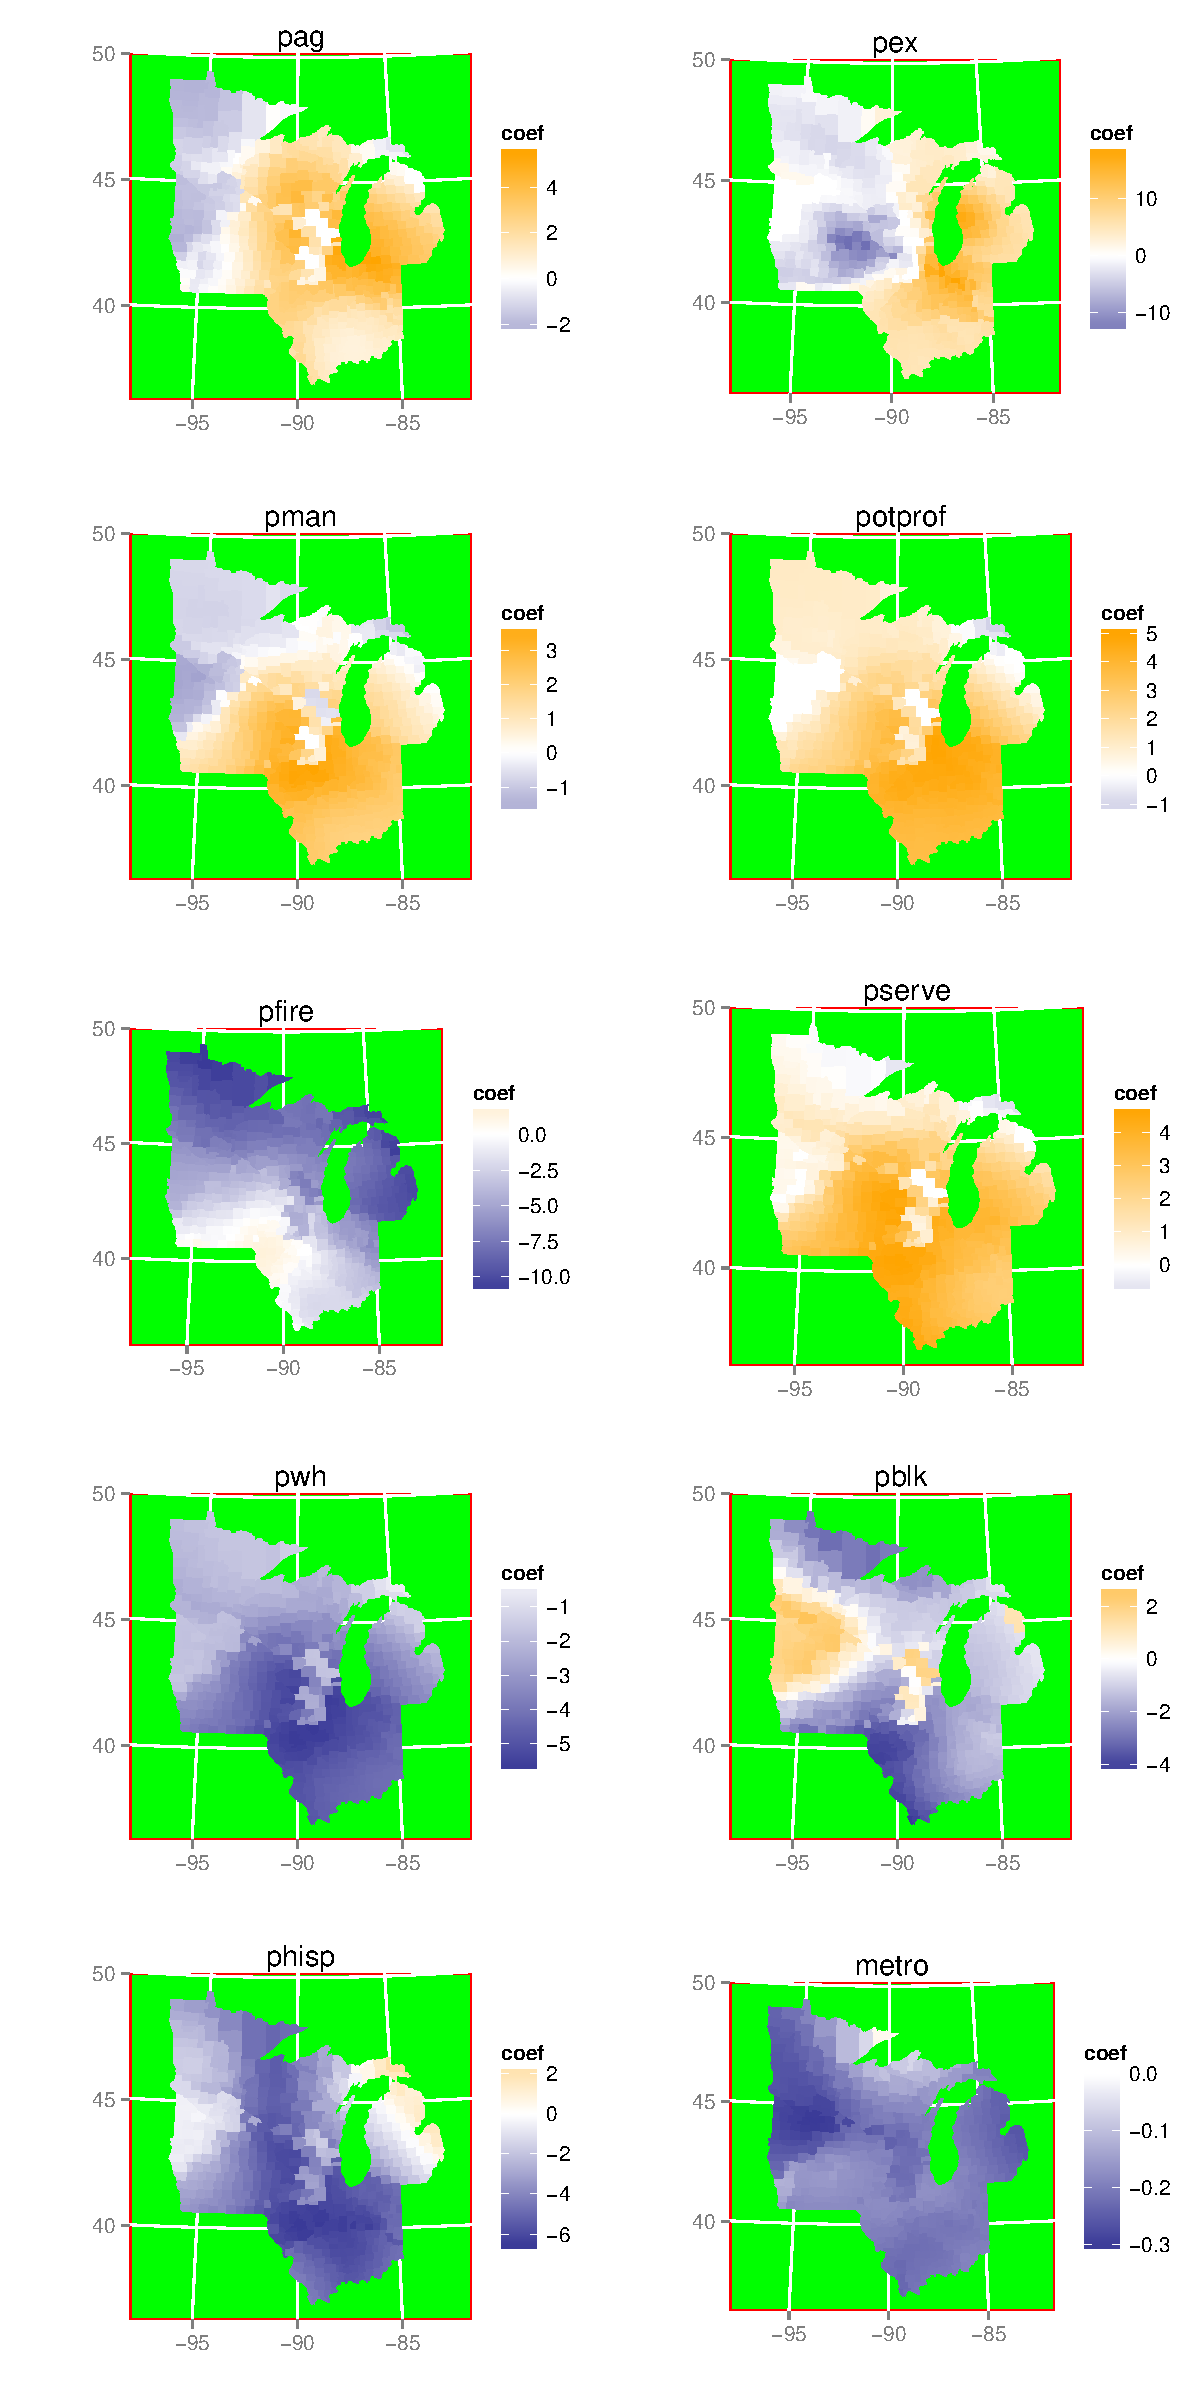
\includegraphics[height=8in]{../../figures/poverty/2006.linear.coefficients.pdf}
			\caption{Estimated coefficient surfaces for the 2006 census.\label{fig:census-coefs-2006}}
		\end{center}
	\end{figure}
			
	\subsection{Discussion}
	If the model is to be believed, then it is onto uncommon for the same variable to have both positive and negative effects on poverty in different geographical areas - see, for instance, the coefficient surface for \verb!pex! (mining employment) in the 1970 census. That surface indicates an interaction whereby the proportion of people working in mining in southern parts of the studied area is associated with an increase in the poverty rate, while in northern parts of the studied area it is associated with a decrease in the poverty rate. Often, a variable is found to be associated with an effect on poverty in some counties but not in others (see, for instance, the coefficient surface for \verb!pserve! (services employment) in 1980 - 
	
	The trend from small bandwidth in the earlier censuses to large bandwidth in the more recent censuses is also interesting - perhaps the local nature 


\section{References}
\bibliographystyle{chicago}
\bibliography{../../references/gwr}

\end{document}  